\documentclass[grad,numbers]{coppe}
\usepackage[utf8]{inputenc}
\usepackage{amsmath,amssymb}
\usepackage{hyperref}

\makelosymbols
\makeloabbreviations



  \RequirePackage[english, brazil]{babel}


\newlength{\cslhangindent}
\setlength{\cslhangindent}{1.5em}
\newenvironment{cslreferences}%
  {}%
  {\par}

\providecommand{\tightlist}{%
  \setlength{\itemsep}{0pt}\setlength{\parskip}{0pt}}
\usepackage{longtable}
\usepackage{booktabs}
\begin{document}
  \title{\emph{Valuation} Intrínseco e Relativo: O estudo de caso da COPEL}
  \foreigntitle{Intrinsic and Relative Valuation: The case study of COPEL}
    \author{Rafael Pinto}{de Freitas}
  
    \advisor{Prof.}{José Roberto}{Ribas}{D.Sc.}
    \advisor{Prof.}{Marco Ludwik Patrício}{Krebs}{D.Sc.}
  

    \examiner{Prof.}{José Roberto Ribas}{D.Sc.}
    \examiner{Prof.}{Marco Ludwik Patrício Krebs}{D.Sc.}
    \examiner{Prof.}{Nome Completo do Terceiro Examinador}{Ph.D}
  
  \department{EPR}
  \date{11}{2020}

    \keyword{Valuation}
    \keyword{Análise de investimentos}
  
  \maketitle

  \frontmatter
  \dedication{\begin{quote}
Judge a man by his questions rather than by his answers.

\hfill --- Voltaire
\end{quote}}
    \chapter*{Agradecimentos}
  Agradeço pela oportunidade de cursar um ensino superior de qualidade de forma pública. Mesmo com suas diversas limitações e imperfeições, a República brasileira segue em frente com a mensagem de democratização do conhecimento. É somente por meio desta que podemos nos defender contra a tirania vil da ignorância. Dessa forma, estou em dívida com a sociedade; com todos que permitiram minha entrada e estadia no curso de Engenharia de Produção pela UFRJ. Uma dívida monumental, se pensada pela ótica dos benefícios. Espero retornar o investimento em breve, a começar de forma humilde com este trabalho de conclusão de curso. Boa leitura!

  Lorem ipsum
  \begin{abstract}
Sit urna lacus aenean euismod morbi integer mauris ligula euismod. Massa leo nunc rutrum non vulputate viverra erat aliquet torquent. Dictumst inceptos litora diam dui eu non sodales eget metus? Mollis faucibus justo class class nulla vestibulum consequat purus.

Sit est ligula massa massa. Lectus parturient vehicula luctus nisl facilisis iaculis sagittis euismod ornare ut platea! Vestibulum et cras nostra luctus morbi cubilia et ante ornare luctus commodo facilisis nam. Lobortis ligula dictum tortor facilisis ante gravida habitasse cras laoreet. Vehicula pharetra vulputate non magna ut interdum habitant quam et class elementum arcu!

Adipiscing nulla laoreet magna dignissim nostra phasellus lacinia elementum est id! Rutrum arcu aliquet torquent porttitor ligula eget dictumst aenean. Lacus dictumst phasellus sed lobortis leo convallis velit mi imperdiet. Ultricies convallis id vestibulum morbi rutrum tortor diam volutpat euismod montes enim cras eros luctus duis rutrum integer.

Consectetur platea augue vitae vitae integer ad tincidunt torquent ac. Pharetra malesuada odio non lobortis dis aliquet arcu nascetur magna porttitor. Lacinia curabitur primis ligula magna sociosqu hendrerit sociosqu risus cubilia. Arcu potenti mi pellentesque nulla per varius vitae lectus pellentesque! Tempor.
  \end{abstract}
  \begin{foreignabstract}
Sit urna lacus aenean euismod morbi integer mauris ligula euismod. Massa leo nunc rutrum non vulputate viverra erat aliquet torquent. Dictumst inceptos litora diam dui eu non sodales eget metus? Mollis faucibus justo class class nulla vestibulum consequat purus.

Sit est ligula massa massa. Lectus parturient vehicula luctus nisl facilisis iaculis sagittis euismod ornare ut platea! Vestibulum et cras nostra luctus morbi cubilia et ante ornare luctus commodo facilisis nam. Lobortis ligula dictum tortor facilisis ante gravida habitasse cras laoreet. Vehicula pharetra vulputate non magna ut interdum habitant quam et class elementum arcu!

Adipiscing nulla laoreet magna dignissim nostra phasellus lacinia elementum est id! Rutrum arcu aliquet torquent porttitor ligula eget dictumst aenean. Lacus dictumst phasellus sed lobortis leo convallis velit mi imperdiet. Ultricies convallis id vestibulum morbi rutrum tortor diam volutpat euismod montes enim cras eros luctus duis rutrum integer.

Consectetur platea augue vitae vitae integer ad tincidunt torquent ac. Pharetra malesuada odio non lobortis dis aliquet arcu nascetur magna porttitor. Lacinia curabitur primis ligula magna sociosqu hendrerit sociosqu risus cubilia. Arcu potenti mi pellentesque nulla per varius vitae lectus pellentesque! Tempor.
  \end{foreignabstract}
  \tableofcontents

  \listoffigures

  \listoftables

  \printlosymbols
  \printloabbreviations

  \mainmatter

  \hypertarget{introduuxe7uxe3o}{%
  \chapter{Introdução}\label{introduuxe7uxe3o}}

  Cabe, antes de começar o desenvolvimento do trabalho propriamente dito, contextualizar e justificar o trabalho, assim como explicitar aos leitores os objetivos, as limitações e a estrutura do mesmo.

  \hypertarget{contextualizauxe7uxe3o}{%
  \section{Contextualização}\label{contextualizauxe7uxe3o}}

  É necessário definir Bolsas de Valores, assim como retratar uma breve história da brasileira a partir de 1967 -- ano a partir do qual começou a se chamar Bolsa de Valores de São Paulo, a Bovespa. Segundo Assaf Neto (\protect\hyperlink{ref-assafneto2018}{2018}), as Bolsas são entidades, cujo objetivo básico é o de manter um local em condições adequadas para a realização de operações de compra e venda de títulos e valores mobiliários.

  Um ano após 1967, foi criado o principal índice de ações brasileiro: o Ibovespa. Resumidamente, este índice é uma média ponderada das ações com maior volume de negociação. Após certo tempo, foi criada a Cetip -- a Central de Custódia e de Liquidação Financeira de Títulos -- em 1984, começando a operar em 1986.

  A partir de 2007, as bolsas de valores deixaram de ser entidades sem fins lucrativos e tornaram-se empresas de capital aberto. No ano seguinte, a BM\&F e a Bovespa se uniram, resultando na criação da Bolsa de Valores, Mercadorias e Futuros de São Paulo -- a BM\&F Bovespa. Em 2017, são fundidas a BM\&F Bovespa e Cetip, dando origem à B3 S.A., sob a supervisão da Comissão de Valores Mobiliários -- esta é a bolsa brasileira atualmente.

  Em tempos contemporâneos, há um crescimento de CPFs registrados na Bolsa de Valores ano a ano, sendo em 2020 o recorde, um aumento de 47.7\% relativo a maio de 2019\footnote{Pode-se conferir a evolução dos mesmos baixando a planilha presente neste link: \url{http://www.b3.com.br/pt_br/market-data-e-indices/servicos-de-dados/market-data/consultas/mercado-a-vista/historico-pessoas-fisicas/}. Último acesso em 07 jul 2020.}.

  Com diversos setores e subsetores de atuação, são diversas as empresas de capital aberto à disposição para escolha do crescente número de investidores brasileiros -- o que não quer dizer que o investidor deve investir em todos. De fato, o investidor precisa minimizar seu risco, preferencialmente investindo em empresas que dentre outras características possuem alto \emph{payout} de dividendos, baixo grau de alavancagem; e menor variabilidade de lucros (BEAVER; KETTLER; SCHOLES, \protect\hyperlink{ref-beaver1970}{1970}).

  Empresas do setor de utilidades possuem tais características, em sua maioria; dessa forma, escolheu-se um exemplar do mesmo -- a Companhia Paranaense de Energia, COPEL -- como forma de fazer o valuation da empresa, fazer um breve resumo do setor elétrico, comparar os métodos de avaliação; e, evidentemente, exemplificar o processo ao leitor.

  \hypertarget{justificativa}{%
  \section{Justificativa}\label{justificativa}}

  Por mais que a caderneta de poupança seja o investimento preferido dos brasileiros, segundo a Associação Brasileira das Entidades dos Mercados Financeiro e de Capitais (\protect\hyperlink{ref-anbima2019}{2019}) -- esta modalidade conta com 88\% da população -- é evidente que o rendimento nominal\footnote{Nominal, pois os retornos reais são contextuais devido ao pagamento de impostos, dividendos; e, a depender do ativo, dos custos do mesmo.} do IBOV é superior no longo prazo. Pelo IPEA, pode-se obter tanto os rendimentos nominais (em \% a.m.) da poupança quanto os retornos do IBOV (também em \% a.m.), ambos em intervalos mensais desde 1990.\footnote{Ambas as séries podem ser obtidas em \url{http://www.ipeadata.gov.br/Default.aspx}. Último acesso em 10 jul 2020.} A partir daí, acumulamos as taxas recursivamente. Definindo \(i\) como a taxa de retorno nominal total, e \(i_t\) como sendo a taxa de retorno nominal no mês \(t\), temos \(i = \prod_{t=1}^n (1+i_t),\) sendo \(n\) o mês que se deseja calcular o retorno nominal total. Exposto isso, foi feito um gráfico dos retornos totais de ambas as modalidades:
  \begin{figure}[H]
  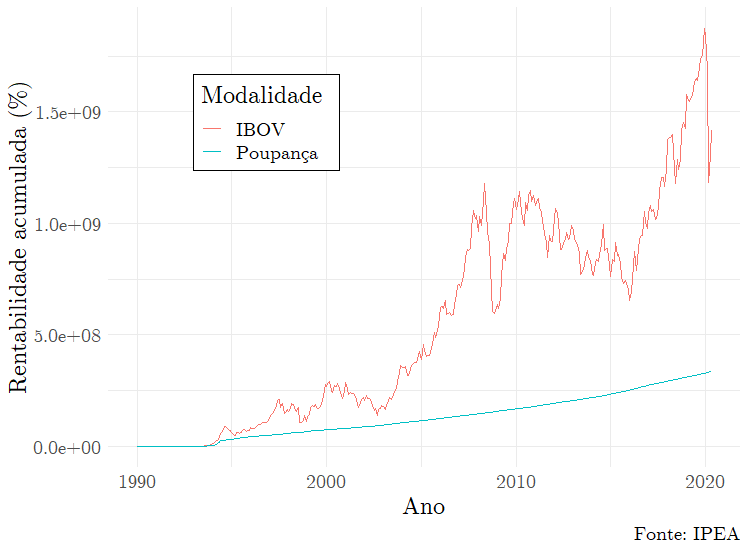
\includegraphics[width=1\linewidth]{img/ibov-poupanca} \caption{Uma comparação entre o IBOV e a poupança.}\label{fig:unnamed-chunk-1}
  \end{figure}
  Com o passar do tempo, entretanto, a maturação no mercado financeiro pode, naturalmente, levar o investidor a se interessar por retornos acima do mercado -- fundos de índice, por definição, impossibilitam o objetivo. Isso leva a uma exploração de diferentes classes de ativos, desde ações ordinárias a fundos de investimento em ações. Um investidor, entretanto, há de ter em mente que raramente fundos de investimento com administração ativa, no longo prazo, superam os retornos dos fundos de índice, em termos reais (BOGLE, \protect\hyperlink{ref-bogle2015}{2015}).

  Assim sendo, caso o investidor deseja ter sucesso, é importante que as escolhas de ativos sejam racionais. Ao menos, tão racionais quanto possível forem para humanos. De fato, indivíduos estão sujeitos a uma racionalidade restrita (SIMON, \protect\hyperlink{ref-simon1997}{1997}), o que leva a diversas heurísticas -- inclusive, mas não limitadas a: enfatizar evidências que apoiam visões próprias (KLAYMAN, \protect\hyperlink{ref-klayman1995}{1995}), superestimar probabilidades por maior ``disponibilidade'' em memória (SCHWARZ et al., \protect\hyperlink{ref-schwarz1991}{1991}); e superestimar a própria habilidade, quando se é novato, assim como subestimar, quando se é um \emph{expert} (KRUGER; DUNNING, \protect\hyperlink{ref-kruger1999}{1999}) -- para simplificar o processo de raciocínio e, permitir, assim, que o agente consiga satisfazer as restrições -- tempo, recursos, dentre outros -- para a tomada de decisões.

  De fato, a abordagem de realizar tanto o \emph{valuation} intrínseco quanto o relativo de uma empresa é, além de uma interessante comparação entre métodos, uma forma de evitar a ``síndrome do homem com martelo'', popularizado por Munger (\protect\hyperlink{ref-munger2006}{2006}). Este cita um provérbio, que diz: ``Para um homem com um martelo, todo problema se parece com um prego.''

  \hypertarget{objetivos}{%
  \section{Objetivos}\label{objetivos}}

  São os principais objetivos do trabalho (1) fazer o \emph{valuation} da Companhia Paranaense de Energia através de, no mínimo, dois métodos de valuation, sendo no mínimo um deles intrísenco e no mínimo, um relativo e (2) realizar a comparação entre os resultados dos métodos.

  Com o desenvolver do trabalho, poderão ser percebidas outras motivações, entretanto seriam estas consideradas secundárias.

  \hypertarget{delimitauxe7uxf5es}{%
  \section{Delimitações}\label{delimitauxe7uxf5es}}

  Este trabalho se limita a prover um breve prospecto do cenário energético brasileiro, assim como possíveis desenvolvimentos. Não serão discutidas políticas energéticas e afins. Se limita, também, a tomar como verdadeira a teoria moderna do portfólio como exposta por Markowitz (\protect\hyperlink{ref-markowitz1952}{1952}), para o cálculo do custo de capital. Não será discutido economia comportamental, nem modelos mais sofisticados para tal cálculo.

  \hypertarget{estrutura-do-trabalho}{%
  \section{Estrutura do trabalho}\label{estrutura-do-trabalho}}

  O trabalho possui, em sua integridade, cinco capítulos.

  O primeiro capítulo é uma introdução ao restante do trabalho, e é efetivamente um resumo do que o leitor verá pela frente.

  O segundo capítulo é uma examinação do setor energético brasileiro, a ser feito pela leitura e examinação do Plano Decenal de Expansão de Energia (PDE) e o Plano Nacioanl de Energia (PNE), ambos elaborados pela Empresa de Pesquisa Energética (EPE). Através destes, podemos ter uma melhor noção do setor no qual a empresa está inserido, possibilitando um melhor cálculo e previsão dos fluxos de caixa.

  O terceiro capítulo é a documentação do referencial teórico utilizado, a ser escrito seguindo uma lógica linear, de forma tal que possa também ser visto como uma metodologia, com exemplos para auxiliar o leitor.

  O quarto capítulo é o estudo de caso de fato. Será dada uma contextualização da empresa, assim como a aplicação dos métodos discutidos.

  O quinto e último capítulo é a conclusão, em que será feita a exposição dos resultados, assim como a comparação entre os métodos de \emph{valuation} discutidos durante o texto.

  \hypertarget{o-mercado-de-energia}{%
  \chapter{O mercado de energia}\label{o-mercado-de-energia}}

  É importante, antes de partir para o estudo de caso em questão, estabelecer o contexto do trabalho em questão. De fato, neste capítulo serão tratados os fundamentais do mercado de energia no Brasil, desde os órgãos aos estudos principais do setor.

  \hypertarget{uxf3rguxe3os-presentes-no-estudo}{%
  \section{Órgãos presentes no estudo}\label{uxf3rguxe3os-presentes-no-estudo}}

  Nesta seção, serão tratados os cinco principais órgãos do setor, sendo eles: (1) o Ministério de Minas e Energia; (2) a Agência Nacional de Energia Elétrica; (3) o Operador Nacional do Sistema Elétrico; (4) a Câmara Comercializadora de Energia Elétrica; e (5) a Empresa de Pesquisa Energética.

  \hypertarget{mme}{%
  \subsection{MME}\label{mme}}

  O Ministério de Minas e Energia (MME) foi criado em 1960, no governo do presidente Juscelino Kubitschek. Assim seguiu por 30 anos, até ser extinto em 1990 e recriado em 1992.

  Em 1997, foi criado o Conselho Nacional de Política Energética (CNPE), vinculado à Presidência da República e presidido pelo ministro de Minas e Energia, com a atribuição de propor ao presidente da República políticas nacionais e medidas para o setor.

  Logo em seguida, em 2003, foram definidas as competências do MME como sendo as áreas de (1) geologia, recursos minerais e energéticos; (2) aproveitamento da energia hidráulica; mineração e metalurgia; e (3) petróleo, combustível e energia elétrica.

  No ano seguinte foi criado o Comitê de Monitoramento do Setor Elétrico (CMSE), cuja função é acompanhar e avaliar permanentemente a continuidade e a segurança do suprimento eletroenergético em todo o território nacional. No mesmo ano, foi permitida também a criação da Empresa de Pesquisa Energética (EPE), vinculada ao Ministério, que tem por finalidade prestar serviços na área de estudos e pesquisas destinadas a subsidiar o planejamento do setor energético.

  O MME tem como empresas vinculadas a Eletrobras e Petrobras. Estão, também, vinculadas algumas autarquias ao Ministério, dentre elas: a Agência Nacional de Energia Elétrica (ANEEL); Agência Nacional do Petróleo, Gás Natural e Biocombustíveis (ANP); e a Agência Nacional de Mineração (ANM).

  \hypertarget{aneel}{%
  \subsection{ANEEL}\label{aneel}}

  A Agência Nacional de Energia Elétrica (ANEEL) é uma autarquia vinculada ao Ministério de Minas e Energia. Tem como finalidade regular e fiscalizar a produção, transmissão, distribuição e comercialização de energia elétrica, de acordo com a legislação e em conformidade com as diretrizes e as políticas do governo federal. A autarquia foi criada em dezembro de 1996, durante o mandato de Fernando Henrique Cardoso.

  Cabe à ANEEL, dentre outras competências: (1) implementar as políticas e diretrizes do governo federal para a exploração da energia elétrica e o aproveitamento dos potenciais hidráulicos; (2) estabelecer as tarifas para o suprimento de energia elétrica realizado às concessionárias e permissionárias de distribuição; e (3) fazer a gestão dos contratos de concessão ou de permisão de serviços públicos de energia elétrica e fiscalizar, diretamente ou mediante convênios com órgãos estaduais, as concessões, as permissões e a prestação dos serviços de energia elétrica.

  Pode-se conferir a lista completa de atribuições pelo Art. 3° da Lei n° 9.427/96.\footnote{Disponível em: \url{http://www.planalto.gov.br/ccivil_03/leis/l9427cons.htm}. Último acesso em 17 nov 2020.}

  \hypertarget{ons}{%
  \subsection{ONS}\label{ons}}

  O Operador Nacional do Sistema Elétrico (ONS) é uma entidade privada sem fins lucrativos que é responsável pela coordenação e controle da operação de instalações de geração e tranmissão de energia elétrica do Sistema Interligado Nacional (SIN), sob fiscalização da ANEEL. O órgão foi criado em agosto de 1998, sob mandato do presidente Fernando Henrique Cardoso.

  \hypertarget{ccee}{%
  \subsection{CCEE}\label{ccee}}

  A Câmara de Comercialização de Energia Elétrica (CCEE) tem por finalidade viabilizar a comercialização de energia elétrica no mercado de energia brasileiro. De fato, esta efetua a contabilização e a liquidação financeira das operações realizadas no mercado de curto prazo. As regras e procedimentos que regulam as atividades realizadas da CCEE são aprovados pela ANEEL.

  Foi criada em agosto de 2004, sob mandato do presidente Luiz Inácio Lula da Silva, sucedendo ao antigo Mercado Atacadista de Energia.

  \hypertarget{epe}{%
  \subsection{EPE}\label{epe}}

  A Empresa de Pesquisa Energética (EPE) é uma empresa pública vinculada ao Ministério de Minas e Energia, criada em março de 2004, sob mandato do presidente Luiz Inácio Lula da Silva. Tem por finalidade prestar serviços na área de estudos e pesquisas destinadas a subsidiar o planejamento do setor energético.

  Cabe à EPE, dentre outras atribuições: (1) apresentar ao CNPE, anualmente, os Planos Decenais de Expansão (PDE), assim como a cada dois anos os Planos Nacionais de Energia (PNE); (2) identificar e quantificar os potenciais de recursos energéticos; e (3) elaborar e publicar o balanço energético nacional.

  A lista completa de atribuições pode ser vista no Art. 4° da Lei n° 10.847/04.\footnote{Disponível em: \url{http://www.planalto.gov.br/CCivil_03/_Ato2004-2006/2004/Lei/L10.847.htm}. Último acesso em 17 nov 2020.}

  Uma das principais motivações para a criação da EPE foram os racionamentos e apagões ocorridos no início da década, ocorridos durante o governo de Fernando Henrique Cardoso, atribuídos em parte á carência de planejamento. Embora seja uma entidade independente, é vinculada ao Ministério de Minas e Energia.

  \hypertarget{o-fluxo-de-energia}{%
  \section{O fluxo de energia}\label{o-fluxo-de-energia}}

  Atualmente, o setor elétrico brasileiro tem uma estrutura predominantemente unidirecional nos fluxos de energia. Assim, são tipicamente dividos em geração, transmissão, comercialização e distribuição. Por se tratarem do final da cadeia de valor convencional, os consumidores então têm efetivamente um comportamento passivo.

  A geração de energia elétrica é a transformação da energia primária -- petróleo, carvão mineral, dentre outros -- em energia elétrica. No Brasil, predomina-se a geração hidráulica devido ao grande potencial hidroenergético dos nossos rios.

  A transmissão efetua o transporte da energia gerada até os centros consumidores de carga. Nessa parte, o sistema brasileiro possui uma particularidade, que é o fato de que os grandes centros de consumidores ficam localizados longe da grande geração energética. Isso faz com que o Brasil tenha uma grande quantidade de linhas de transmissão com algumas centenas de quilômetros.

  A comercialização de energia é atualmente realizada em dois ambientes diferentes: (1) no Ambiente de Contratação Livre, que é destinado ao atendimento de consumidores livres -- o consumidor que pode optar pela compra de energia elétrica junto a qualquer fornecedor, que é atendido em qualquer tensão e com demanda contratada mínima de 3 MW, segundo a Resolução da ANEEL n° 376, de 25 de agosto de 2009\footnote{Disponível em: \url{https://www.legisweb.com.br/legislacao/?id=109898}. Último acesso em 17 nov 2020.} e a Resolução n° 414, de 9 de setembro de 2010\footnote{Disponível em: \url{https://www.legisweb.com.br/legislacao/?id=112868}. Último acesso em 17 nov 2020.}; e (2) no Ambiente de Contratação Regulada, que é destinado ao atendimento de consumidores cativos por meio das distribuidoras, sendo estas supridas por geradores estatais ou independentes que vendem energia em leilões públicos.

  A distribuição é o setor responsável por receber a energia da transmissão e distribuí-la para os centros consumidores.

  Salvo no caso de \emph{holdings}, empresas só podem atuar em uma das áreas ex-comercialização.

  \hypertarget{estudos-e-projeuxe7uxf5es-de-longo-prazo}{%
  \section{Estudos e projeções de longo prazo}\label{estudos-e-projeuxe7uxf5es-de-longo-prazo}}

  A EPE cumpre sua finalidade de braço técnico de estudos do setor energético produzindo relatórios e planos de expansão a respeito do setor elétrico. Por se tratar de um \emph{valuation} de uma empresa do setor, é importante ponderar a respeito das ações tomadas e o parecer de \emph{experts} a respeito do futuro do setor como um todo, a fim de aprimorar nossas estimativas da taxa de crescimento.

  São os dois principais estudos, nesse sentido, (1) o Plano Nacional de Energia; (2) e o Plano Decenal de Expansão de Energia

  \hypertarget{plano-nacional-de-energia-pne}{%
  \subsection{Plano Nacional de Energia (PNE)}\label{plano-nacional-de-energia-pne}}

  O PNE é um conjunto de estudos que dão suporte ao desenho da estratégia de longo prazo do governo em relação à expansão do setor de energia. A estratégia, por sua vez, consiste em um conjunto de recomendações e diretrizes a serem seguidas na definição das ações e iniciativas a serem implementadas ao longo do horizonte de tempo prescrito. A revisão do PNE deve ser conduzida sempre que houver necessidade de alteração na estratégia de longo prazo do tomador de decisão relevante, sejam por razões ordinárias ou extraordinárias.

  Os PNEs têm relação com os PDEs. Embora haja similaridades, o PNE é um instrumento de planejamento com atribuições distintas do PDE. Em primeiro lugar, o PNE é um documento com visão mais estratégica. Neste contexto, seu enfoque consiste em embasar o posicionamento do governo de modo a orientar e direcionar as estratégias dos agentes do setor de forma a se atingir os objetivos gerais da expansão no longo prazo, com adequação dos recursos, com confiabilidade, modicidade e sustentabilidade. Além disso, o PNE é o alicerce a partir de qual todos os Planos, Políticas, Programas e Iniciativas são elaborados. O PNE é, portanto, um farol que orienta para onde os PDEs devem indicar a expansão do setor de energia no horizonte decenal. Por fim, enquanto o PDE trabalha com um cenário de referência e análises de sensibilidade, anualmente revisto, o PNE deve tratar com mais cenários.

  No caso, foi feito o estudo do PNE 2050 (EPE, \protect\hyperlink{ref-epe2020}{2020}), e assim será entregue um pequeno sumário executivo do mesmo a seguir.

  Foram elaborados dois grandes cenários, formando um cone de incertezas para o desenho da estratégia de longo prazo: o primeiro, chamado Desafio da Expansão, reflete requisitos de expansão do setor de energia para atendimento a um crescimento da demanda de energia mais expressivo. No segundo, chamado de Estagnação, analisam-se as consequências de um cenário em que o consumo de energia per capita mantém-se inalterado ao longo de todo o período. O foco do relatório está voltado para o cenário Desafio da Expansão.

  Os estudos do PNE apontam para um potencial energético de quase 280 bilhões de tep (toneladas equivalentes de petróleo) no horizonte até 2050. A demanda cresce de 300 milhões de tep para 600 milhões de tep e, ao longo de trinta e cinco anos, essa trajetória representa uma demanda de energia total acumulada do período equivalente a pouco menos de 15 bilhões de tep. Tamanha discrepância entre potencial de recursos e a demanda de energia estimada gera uma situação distinta daquela vivida ao longo especialmente da metade do século XX, quando o País viveu grandes crises de energia. Dessa forma, imagina-se uma administração da abundância.

  O cenário Desafio da Expansão considera algumas premissas, que serão levadas em conta para o uso no estudo de caso. São essas: (1) crescimento médio de PIB de 3.1\% a.a. e 2.8\% de PIB per capita; (2) a população brasileira manterá a tendência de crescer a taxas cada vez menores; (3) o consumo potencial de energia elétrica do País pode atingir até 3 vezes o patamar do ano base; (4) a demanda de energia elétrica a ser atendida por geração centralizada cresce até 2.5 vezes em relação aos valores do ano base, mesmo com crescimento de geração distribuída (GD), autoprodução, energia solar térmica e eficiência energética no período; (5) e o consumo de energia e de eletricidade per capita aumenta, a despeito da contribuição da eficiência energética no horizonte até 2050.

  \hypertarget{plano-decenal-de-expansuxe3o-de-energia-pde}{%
  \subsection{Plano Decenal de Expansão de Energia (PDE)}\label{plano-decenal-de-expansuxe3o-de-energia-pde}}

  O PDE tem o intuito de de indicar as perspectivas, sob a ótica do Governo, da expansão do setor de energia no horizonte de dez anos, dentro de uma visão integrada para os diversos energéticos. Tal visão permite, então, extrair importantes elementos para o planejamento do setor, com benefícios em termos de aumento de confiabilidade, redução de custos de produção e mitigação de impactos ambientais.

  Como o PDE tem intuitos mais operacionais do que estratégicos, serão utilizadas as premissas e estudos do PNE para nortear as decisões do presente \emph{valuation}.

  \hypertarget{referencial-teuxf3rico}{%
  \chapter{Referencial teórico}\label{referencial-teuxf3rico}}

  Nesta seção será feita uma consideração a respeito dos métodos e conceitos utilizados ao longo do estudo. É de interesse do leitor prestar especial atenção ao enunciado abaixo, uma vez que é um breve alicerce teórico que serve não apenas para esse estudo, como para diversos outros similares. Recomenda-se, ainda, a leitura de Damodaran (\protect\hyperlink{ref-damodaran2007}{2007}) para se ter um panorama de diversos outros modelos a serem aplicados, assim como uma discussão a respeito de seus usos e efetividade.

  \hypertarget{valuation-intruxednseco}{%
  \section{\texorpdfstring{\emph{Valuation} intrínseco}{Valuation intrínseco}}\label{valuation-intruxednseco}}

  Comecemos discutindo brevemente a respeito do que é possuir ``valor intrínseco''. Este é um conceito filosófico, em que o valor de um objeto ou projeto é derivado de, e por si só -- em outras palavras, livre de fatores externos. Analistas financeiros constroem modelos para estimar o que se imagina ser o valor intrínseco de uma empresa sem considerar o seu valor de mercado em determinado dia.

  Naturalmente, o mercado, no curto prazo, está sujeito a flutuações que podem ser atribuídas a diversos fatores, desde manipulação de preços em papéis mais ilíquidos a pensamento de manada por parte de investidores. Cabe, nesse momento, utilizar a analogia popularizada por Graham (\protect\hyperlink{ref-graham2016}{2016}, pp.~204-205), do Sr.~Mercado:
  \begin{quote}
  ``Imagine que você possui uma participação pequena em uma companhia de capital fechado que lhe custou US\$1.000. Um de seus sócios, chamado Sr.~Mercado, é de fato muito prestativo. Todo dia ele lhe informa o que pensa ser o valor de sua participação e, além disso, se dispõe a comprar de você ou vender a você uma participação adicional naquelas bases. Às vezes, sua ideia de valor parece plausível e justificada pela evolução e pelas perspectivas do negócio da forma como você as conhece. Por outro lado, o Sr.~Mercado deixa frequentemente o entusiasmo ou o receio tomar conta dele e o valor proposto por ele lhe parece pura bobagem. Se você é um investidor prudente ou um empresário inteligente, deixaria as comunicações diárias do Sr.~Mercado influenciarem sua opinião sobre o valor de uma participação de US\$1.000 na companhia? Só se você concordasse com ele ou então desejasse negociar com ele. Você pode ficar feliz em vender para ele quando ele cota um preço ridiculamente alto e igualmente feliz em comprar dele quando seu preço é baixo. No entanto, no resto do tempo, você seria mais esperto se formulasse suas próprias ideias acerca do valor de sua carteira com base nos relatório completos da companhia sobre suas operações e posições financeiras.''
  \end{quote}
  Dessa forma, a discrepância entre preço de mercado e a estimativa do valor intrísenco feita por um analista torna-se uma medida para oportunidade de investimento. Aqueles que considerarem tais modelos como estimativas razoáveis de valor intrínseco, e que tomarem ação baseando-se nessas estimativas, são conhecidos como investidores de valor (DAMODARAN, \protect\hyperlink{ref-damodaran2012}{2012}).

  \hypertarget{anuxe1lise-de-fluxo-de-caixa-descontado}{%
  \subsection{Análise de Fluxo de Caixa Descontado}\label{anuxe1lise-de-fluxo-de-caixa-descontado}}

  A análise de fluxos de caixa descontados (DCF) é um método de se descobrir o valor de uma ação, projeto, empresa, ou ativo usando os conceitos do valor temporal do dinheiro. Para se aplicar o método, todos os fluxos de caixa futuros são estimados e descontados ao se utilizar o custo de capital para dar seus valores presentes. A soma de todos os futuros fluxos de caixa, tanto de entrada quanto de saída, resulta no valor presente líquido, que é tomado como o valor dos fluxos de caixa em questão, no momento.

  Seguindo a queda do mercado em 1929, o método ganhou popularidade para se avaliar ações. De fato, provavelmente o primeiro a formalizar a expressão do método em termos econômicos modernos foi Fisher (\protect\hyperlink{ref-fisher1930}{1930}).

  O valor presente líquido pode ser expresso matematicamente como: \[
  VPL = \sum_{i=0}^N\frac{FC_t}{(1+r)^t}
  \] onde \(FC_t\) é o fluxo de caixa no tempo \(t\) e \(r\) é a taxa de desconto. Naturalmente, para que o somatório acima esteja correto, assume-se que a taxa de desconto permaneça constante através do período todo. Caso assuma-se que o fluxo de caixa continue indefinidamente, a previsão finita é geralmente combinada com a premissa de um crescimento constante de fluxo de caixa além do período de projeção discreto -- a dita perpetuidade. Matematicamente: \[
  VPL = \sum_{i=0}^N\frac{FC_t}{(1+r)^t} + \frac{FC_{N+2}}{(1+r)^{N+1}(r-g)}
  \] onde o somatório é o período de crescimento normal, e além do somatório, temos o fluxo de caixa em perpetuidade, sendo descontado.

  A pergunta, entretanto, repousa sobre encontrar a taxa de desconto. Diversos modelos foram apresentados com tal finalidade, sendo o mais utilizado o \emph{capital asset pricing model}, doravante mencionado pela sua abreviatura, CAPM.

  Este modelo foi introduzido por Sharpe (\protect\hyperlink{ref-sharpe1964}{1964}), desenvolvendo em cima do trabalho iniciado em diversificação e teoria moderna do portfólio (MARKOWITZ, \protect\hyperlink{ref-markowitz1952}{1952}). O CAPM leva em conta a sensibilidade de um ativo ao risco não diversificável -- também conhecido como risco sistemático, ou risco de mercado -- geralmente representado por \(\beta\). De fato, a equação é como segue: \[
  E(R_i) = R_f + \beta_i(E(R_m)-R_f)
  \] onde \(E(R_i)\) é o retorno esperado do ativo, \(R_f\) é a taxa de juros livre de risco -- oriunda geralmente de títulos do governo -- e \(E(R_m)\) é o retorno esperado do mercado. \(\beta\), como comentado, é a sensibilidade do ativo em relação ao mercado, de forma tal que: \[
  \beta_i = \frac{Cov(R_i, R_m)}{Var(R_m)} = \rho_{i,m}\frac{\sigma_i}{\sigma_m}
  \] onde \(\rho_{i,m}\) denota o coeficiente de correlação entre o investimento \(i\) e o mercado \(m\), \(\sigma_i\) é o desvio padrão para o investimento \(i\), e \(\sigma_m\) é o desvio padrão para o mercado \(m\).

  Podemos entender essa equação melhor se a rearranjarmos: \[
  E(R_i) = R_f + \beta_i(E(R_m)-R_f) \iff E(R_i) - R_f = \beta_i(E(R_m)-R_f)
  \] onde o segundo lado denota uma equivalência interessante. Dessa forma, podemos dizer que o prêmio de risco para o ativo individual é igual ao prêmio pelo risco de mercado, multiplicado pela sensibilidade do ativo (\(\beta\)).

  De fato, o modelo leva em conta diversas premissas, dentre as quais todos os investidores (ARNOLD, \protect\hyperlink{ref-arnold2008}{2008}):
  \begin{enumerate}
  \def\labelenumi{\arabic{enumi}.}
  \tightlist
  \item
    Têm por objetivo maximizar utilidades econômicas (quantidades de ativos são dadas e fixas).
  \item
    São racionais e aversos a risco.
  \item
    São amplamente diversificados sobre uma grande gama de investimentos.
  \item
    São tomadores de preço, isto é, não influenciam nos preços.
  \item
    Podem emprestar e tomar quantias ilimitadas sob a taxa livre de risco de juros.
  \item
    Fazem trocas sem custo de transação ou impostos.
  \item
    Lidam com ativos que são todos altamente diversificáveis em pequenas parcelas -- são perfeitamente divisíveis e líquidos).
  \item
    Têm expectativas homogêneas.
  \item
    Têm todas as informações disponíveis ao mesmo tempo.
  \end{enumerate}
  Naturalmente, pela quantidade e teor das premissas, este é um modelo que fortemente simplifica a realidade. De fato, pela sua lógica simples e fácil aplicabilidade, ainda é muito utilizado na indústria, embora a maior parte das aplicações utilizando-se este modelo sejam consideradas inválidas (FAMA; FRENCH, \protect\hyperlink{ref-fama2004}{2004}).

  Para os propósitos deste trabalho, entretanto, será feita uma análise de fluxos de caixa descontados utilizando-se, também, o CAPM.

  \hypertarget{modelo-de-desconto-de-dividendos}{%
  \subsection{Modelo de Desconto de Dividendos}\label{modelo-de-desconto-de-dividendos}}

  O modelo de desconto de dividendos (DDM) é um método de se fazer o \emph{valuation} de uma ação baseado na teoria de que a ação vale a soma de todos os seus pagamentos de dividendos futuros, descontados de volta ao seu valor presente líquido (VPL). A equação mais utilizada amplamente é o chamado modelo de crescimento de Gordon (GGM). É nomeada assim por causa da publicação de Gordon e Shapiro (\protect\hyperlink{ref-gordon1959}{1959}), embora tenha sido originalmente desenvolvida três anos antes (GORDON; SHAPIRO, \protect\hyperlink{ref-gordon1956}{1956}). Trata-se da equação: \[
  P_0 = \frac{D_1}{r-g}
  \] onde \(P_0\) é o valor atual da ação, \(g\) é a taxa de crescimento constante em perpetuidade esperada dos dividendos, \(r\) é o custo de capital próprio da empresa; e \(D_1\) é o valor dos dividendos do próximo ano.

  Naturalmente, existem alguns pressupostos deste modelo:
  \begin{enumerate}
  \def\labelenumi{\roman{enumi}.}
  \tightlist
  \item
    Uma taxa de crescimento constante e perpétua, menor que o custo de capital.
  \item
    A ação deve pagar dividendos regularmente; do contrário, versões mais generalizadas do modelo de desconto de dividendos devem ser usados para se descobrir o valor da ação.
  \end{enumerate}
  A partir destes pontos, temos que as violações de (i) identifica uma ação de valor negativo; e (ii) provê um valor errôneo -- caso seja levado ao extremo, uma empresa que não paga dividendos efetivamente não valeria nada.

  A solução para (i) é se considerar um modelo de desconto de dividendos de dois estágios, isto é: \[
  P_0 = \frac{D_0 (1+g)}{r-g} \left[1 - \frac{(1+g)^N}{(1+r)^N}\right] + \frac{D_0 (1+g)^N (1+g_\infty)}{(1+r)^N (r-g_\infty)}
  \] onde \(D_0\) denota os dividendos deste ano, \(g\) a taxa de crescimento esperada de curto prazo, \(g_\infty\) a taxa de crescimento de longo prazo, e \(N\) o período (em número de anos), através do qual a taxa de curto prazo é aplicada.

  Uma solução comum para (ii) seria assumir que a hipótese de Modigliani-Miller de irrelevância de dividendos (MODIGLIANI; MILLER, \protect\hyperlink{ref-modigliani1958}{1958}) seja verdadeira, e então substituir os dividendos \(D\) por \(E\), os lucros por ação. Entretanto, isso requer o uso de crescimento dos lucros, ao invés dos de dividendos, que podem ser diferentes.

  A equação de Gordon pode ser entendida como o fato de que o retorno total de uma ação é igual à soma da sua receita e seus ganhos de capital. De fato, se rearranjada, teremos que: \[
  P_0 = \frac{D_1}{r-g} \iff \frac{D_1}{P_0} + g = r
  \] o que significa que o \emph{dividend yield} (\(D_1/P_0\)) mais o crescimento (\(g\)) é igual ao custo de capital próprio (\(r\)). Ora, caso consideremos a taxa de crescimento de dividendos no modelo como um \emph{proxy} para o crescimento de lucros e, por extensão, o preço da ação e os ganhos de capital. Consideraríamos, então, o custo de capital próprio como um \emph{proxy} para o retorno total requerida pelo investidor.

  \hypertarget{valuation-relativo}{%
  \section{\texorpdfstring{\emph{Valuation} relativo}{Valuation relativo}}\label{valuation-relativo}}

  Em \emph{valuation} relativo, um determinado ativo é avaliado baseado em quão precificados estão os ativos similares no mercado. Como exemplo, uma comprador de imóveis pode, antes de realizar uma compra à vista/financiamento abrupto, pode pesquisar por imóveis similares na vizinhança. Ora, uma pessoa que coleciona selos pode fazer um julgamento de quanto vai pagar em outro selo raro ao checar preços de transações desse mesmo selo em outras épocas. Dessa forma, um investidor em potencial pode estimar o preço de uma ação a comprar fazendo uma pesquisa através da precificação de ações ``similares''.

  Pela descrição acima, existem três fatores a se considerar:
  \begin{enumerate}
  \def\labelenumi{\arabic{enumi}.}
  \tightlist
  \item
    \textbf{É necessário encontrar ativos comparáveis, precificados pelo mercado.} Esta é uma tarefa que é mais fácil de se cumprir com ativos tangíveis do que com imateriais, como ações. Frequentemente, analistas consideram outras empresas do mesmo setor como comparáveis, comparando por exemplo, empresas de utilidade com outras empresas de utilidade.
  \item
    \textbf{É importante traduzir os preços de mercado a uma variável comum.} A finalidade disso é gerar preços padronizados que sejam comparáveis. Embora isso não seja necessário com ativos idênticos, é necessário quando existe heterogenia. Considere, por exemplo, o exemplo dos imóveis. Uma casa tem 200 m² e outra, 100 m². Reduziria-se um fator à metragem. Naturalmente, com empresas acontece algo similar, geralmente reduzindo-se a múltiplos de lucros, valor contábil, dentre outros.
  \item
    \textbf{É necessário ajustar-se diferenças entre ativos.} Novamente, consideremos o exemplo da casa. Ambas possuem a mesma metragem, mas uma acabou de ser construída, e outra tem mais de 200 anos de idade. Ora, havendo essa diferença de idades, \emph{ceteris paribus}, a casa mais nova deve valer mais. Com ações, pode haver algo similar. Empresas de maior crescimento, \emph{ceteris paribus}, devem valer mais do que empresas de menor crescimento, por exemplo.
  \end{enumerate}
  Cabe comentar que existe uma diferença filosófica significativa entre as abordagens intrínseca e relativa. Através de \emph{valuation} intrínseco, tentamos estimar o valor de um ativo baseado na sua capacidade de gerar fluxos de caixa no futuro. No \emph{valuation} relativo, estamos fazendo um julgamento em quanto um ativo vale ao olharmos para o que o mercado está pagando por ativos similares -- implicitamente, estamos ``confiando'' no julgamento de valor do mercado. Dessa forma, caso o mercado esteja sistematicamente superestimando ou subestimando -- \emph{bull} e \emph{bear market}, respectivamente -- um grupo de ativos ou um setor inteiro, ambos os tipos de \emph{valuation} podem diferir entre si.

  \hypertarget{anuxe1lise-por-muxfaltiplos}{%
  \subsection{Análise por múltiplos}\label{anuxe1lise-por-muxfaltiplos}}

  Múltiplos, efetivamente, são uma tentativa de reduzir empresas a ``fatores comuns'', para que possam ser feitas comparações tão precisas quanto possíveis. No geral, valores podem ser padronizados relativo aos lucros que as firmas geram, aos valores contábeis; ou valores de substituição das firmas em si mesmas, às receitas que firmas geram, ou para medidas que são específicas para as firmas em um setor.

  Pelo interesse de se desenvolver melhores ferramentas de filtragem, o estudo de tais indicadores foi iniciado. Vale, então, comentar a respeito da precisão histórica de tais múltiplos.

  Existiram, naturalmente, estudos que relacionaram múltiplos com fundamentais de \emph{valuation} (BEAVER; MORSE, \protect\hyperlink{ref-beaver1978}{1978}; PEASNELL, \protect\hyperlink{ref-peasnell1982}{1982}). De fato, há uma forte conexão entre o valor contábil e retorno sobre patrimônio líquido, como notado por Wilcox (\protect\hyperlink{ref-wilcox1984}{1984}), fazendo o argumento de que ações baratas são aquelas que são vendidas a múltiplos de valor contábil baixos enquanto mantém retornos sobre o patrimônio líquidos altos ou, no mínimo, razoáveis. Na verdade, Penman (\protect\hyperlink{ref-penman1996}{1996}) também traça uma distinção entre múltiplos de preço sobre lucro e múltiplos de valor contábil no que tange a sua ligação com o retorno sobre o patrimônio líquido, ao mencionar que, à medida que múltiplos de PBV aumentam com o ROE, a relação entre múltiplos de P/L e ROE é mais fraca. Múltiplos de lucros por ação são os melhores em explicar diferenças em precificação, múltiplos de vendas e fluxos de caixa operacionais são os piores, e múltiplos de valor contábil e EBITDA tendem a ficar no meio (LIE; LIE, \protect\hyperlink{ref-lie2002}{2002}; LIU; NISSIM; THOMAS, \protect\hyperlink{ref-liu2002}{2002}, \protect\hyperlink{ref-liu2007}{2007}). Curiosamente, existe ainda uma relação inversa entre volatilidade do mercado e múltiplos de P/L (STOHS; MAUER, \protect\hyperlink{ref-stohs1996}{1996}), demostrando a aversão ao risco do investidor.

  \hypertarget{estudo-de-caso}{%
  \chapter{Estudo de caso}\label{estudo-de-caso}}

  Iniciamos, agora, o estudo do caso propriamente dito -- sendo este o da Companhia Paranaense de Energia. Para um estudo próprio de \emph{valuation}, é necessário conhecer-se o ativo a ser estudado. Isso com a finalidade de poder realizar estimativas de crescimento e risco mais apropriadas, assim como realizar um pequeno dossiê da empresa e suas conquistas, elucidando assim práticas de governança e um histórico operacional.

  \hypertarget{breve-dossiuxea-da-copel}{%
  \section{Breve dossiê da COPEL}\label{breve-dossiuxea-da-copel}}

  Comecemos, desta forma, fazendo um dossiê da empresa, de forma a estudar melhor sua história e operações, assim como expor casos relevantes da empresa.

  \hypertarget{histuxf3ria}{%
  \subsection{História}\label{histuxf3ria}}

  É de suma importância comentar que a parte a seguir é uma adaptação de transcritos oriundos do site da própria empresa,\footnote{Versão completa disponível em: \url{https://www.copel.com/hpcopel/root/nivel2.jsp?endereco=\%2Fhpcopel\%2Froot\%2Fpagcopel2.nsf\%2Fdocs\%2F6505401715872FAA032573FA0069734F}. Último acesso em 10 nov 2020.} com pequenos acréscimos por parte do autor.

  A Companhia Paranaense de Energia é a maior empresa do estado do Paraná, tendo sido criada em 26 de outubro de 1954, sob controle acionário do estado do Paraná, abrindo seu capital acionário em abril de 1994 na BM\&FBovespa, e tornou-se em julho de 1997 a primeira do setor elétrico brasileiro a ser listada na Bolsa de Valores de Nova Iorque. A marca está também presente, desde junho de 2002, na Comunidade Econômica Europeia, pela Latibex -- o setor latinoamericano da Bolsa de Valores de Madri. A partir de 7 de maio de 2008, a empresa também passou a figurar oficialmente no Nível 1 de Governança Corporativa da BM\&FBovespa.

  Em 2017, a Companhia atendia diretamente a mais de 4,5 milhões de unidades consumidoras em quase 400 municípios e 1.113 localidades paranaenses. Nesse universo incluem-se 3,6 milhões de lares, 78 mil indústiras, 384 mil estabelecimentos comerciais e 356 mil propriedades rurais. O quadro de pessoal, na época, era integrado por 8.453 empregados.

  Sua estrutura compreende a operação de:
  \begin{itemize}
  \tightlist
  \item
    Parque gerador próprio composto por 30 usinas próprias e 11 participações, cuja potência instalada totaliza 5.675 MW -- a maior parte proveniente de fontes renováveis como hídrica e eólica -- e que responde pela produção de aproximadamente 4\% de toda a eletricidade gerada no Brasil.
  \item
    Sistema de transmissão formado por mais de 4 mil km de linhas e 45 subestações automatizadas.
  \item
    Sistema de distribuição com 195 mil km de linhas -- a terceira maior do País -- e 362 subestações automatizadas.
  \end{itemize}
  Hoje as usinas, linhas de transmissão e de distribuição da Copel transmitem luz para todo o Paraná e estados vizinhos. Tal cenário de progresso tem sido conquistado ao longo de seis décadas, com base no potencial hidráulico e no domínio tecnológico de seus quadros técnicos e profissionais.

  Comentemos, agora, uma breve linha do tempo da Companhia.

  Foi criada a Copel -- ainda Companhia Paranaense de Energia Elétrica -- através do Decreto n° 14.947 de 26 de outubro de 1954, assinado por Bento Munhoz da Rocha Neto, na época governador do Paraná. Apenas em 1979 tornou-se Companhia Paranaense de Energia, tendo como base principal para a integralização de seu capital o Fundo Estadual de Eletrificação. Em seguida, em 1956, com o Decreto n° 1.412, a Copel passou a centralizar todas as ações governamentais de planejamento, construção e exploração dos sistemas de produção, transmissão, transformação, distribuição e comércio de energia elétrica e serviços correlatos, tendo incorporado, de forma central, todos os bens, serviços e obras em poder de diversos órgãos. Coube à Companhia, então, ser responsável pela construção dos grandes sistemas de integração enerética e dos empreendimentos hidrelétricos previstos no Plano de Eletrificação do Paraná. Inclusive, no mesmo ano, em 1° de agosto, a Companhia assumiu pela primeira vez o serviço de distribuição de energia de um munícip do estado: Maringá. Na época, Maringá possuía um rápido crescimento demográfico. Ora, com a chegada da Copel e da energia elétrica, o desenvolvimento do municípío acelerou ainda mais. Em seguida, vieram outros municípios.

  Durante a década de 60 e 70, pode-se constatar que o maior desafio para a Copel foi encontrar uma solução definitiva para o abastecimento de energia elétrica em larga escala. De fato, iniciaram-se as operações em 1963 da Usina Termelética de Figueira, de fundamental importância para a implantação do Plano Estadual de Eletrificação, viabilizando os sistemas de interligação que beneficiaram as Regiões Norte e Centro. Quatro anos depois, a Copel inaugurava a Usina de Salto Grande do Iguaçu, para atender ao sul do Estado. Entrando na década de 70, entrava em operação a Usina Julio de Mesquita Filho, para abastecer energicamente o oeste e o sudoeste. Um ano após, foi inaugurada a Usina Governador Parigot de Souza, este nome sendo uma homenagem ao governador Pedro Viriato Parigot de Souza, que também tinha sido presidente da Copel. É, atualmente, a maior central subterrânea do sul do Brasil e era a principal unidade geradora da Copel e maior usina em funcionamento no sul do Brasil no momento de sua inauguração, sendo um passo definitivo na constituição de uma infraestrutura energética capaz de suportar o desenvolvimento paranaense.

  Nos anos de 1973 e 1974, a Copel deu um salto no número de consumidores ao assumir a distribuição de energia de diversos municípios do Estado. Em 1° de agosto de 1973, a Companhia incorporava a Companhia Força e Luz do Paraná, que atendia Curitiba. Um ano após, em 1° de junho de 1974, a Copel assumiu, também a distribuição de Londrina. Aliado a isso, foi lançado um programa de inclusão elétrica pela empresa, o que contribuiu para levar energia a ainda mais residências. Dessa forma, tivemos em 1981 a marca de 1 milhão de consumidores ligados à rede.

  Naturalmente, com tamanha expansão de clientela, seria necessário à empresa expandir sua capacidade energética. Dessa forma, em 1980 foi inaugurada a hidrelétrica Governador Bento Munhoz da Rocha Netto, nomeada em honra ao governador Bento Munhoz da Rocha Netto, governador este que assinou o Decreto para a criação da Companhia. Com essa operação, a geração própria da Copel atingiu 2.9 bi kWh, contra 1.9 bi kWh do ano anterior.

  1986 foi um ano de retrospectiva para a Companhia. De fato, ela levou 27 anos (de 1954 a 1981) para alcançar 1 milhão de consumidores, e somente 5 anos para aumentar outros 500 mil. Essa conquista, inclusive, se deu em meio ao racionamento de energia por causa de uma estiagem forte na região. Assim sendo, as décadas seguintes são marcadas por uma expansão exponencial da empresa, assim como um aumento das obras para se expandir a capacidade energética.

  Em setembro de 1992, foi concluída a Usina Hidrelétrica Governador Ney Aminthas de Barros Braga. Contribuiu para reduzir a dependência paranaense de energia comprada de outros Estados. Foi, inclusive, a primeira usina hidrelétrica a ter um Relatório de Impacto Ambiental (RIMA). Em fevereiro de 1999, entra em operação a Usina Hidrelétrica Governador José Richa.

  Em 2004, a Copel completou 50 anos de existência. Apenas dois anos antes, foi anunciado o cancelamento do processo de privatização da Companhia, iniciado em 1998. Com o passar dos anos, a empresa se tornou expoente no que tange a P\&D do setor elétrico, com diversas inovações. Nota-se, por exempo, o marco do funcionamento da primeira célula a combustível a operar no Hemisfério Sul, em 2001, para suprir o CPD da Copel. Houve também a automação da subestação Jardim Tropical, fazendo com que a empresa sae tornasse a primeira do setor elétrico brasileiro a automatizar todas as subestações de transmissão.

  A empresa inaugura, em 2 anos, 2 novas hidreléticas: a de Santa Clara e a do Fundão. No meio tempo da construção de outra usina, ambas Santa Clara e Fundão recebem autorização da ONU e tornam-se as primeiras hidreléticas do Brasil a poderem comercializar certificados de Créditos de Carbono. De fato, existem duas outras usinas com planos de construção, a de Mauá e a Colíder, demonstrando assim a demanda de expansão da Companhia.

  Em 2012, a Copel finalizou todas as fases do programa Luz para Todos, efetivamente conquistando a universalização do fornecimento de energia elétrica no Paraná. O reconhecimento foi formalizado pela ANEEL, marcando assim o início de uma era sob motivação de modernização e automação das redes de energia por parte da empresa. Três anos após, em janeiro, a Copel institui uma empresa de comercialização para atuar no Mercado Livre, atuando assim na compra e venda de energia, além de consultoria. A partir de 2016, a empresa volta seus esforços para além do Paraná, com entradas de operação em linhas de transmissão de conectam o Paraná ao Mato Grosso e um no Maranhão.

  Podemos notar, então, um grau de maturidade elevado por parte da empresa atualmente, em que a mesma segue uma motivação de melhoria dos processos atuais, com objetivo secundário de ampliar para outros estados, à medida que concessões e órgãos reguladores dão seu aval.

  \hypertarget{core-business}{%
  \subsection{\texorpdfstring{\emph{Core business}}{Core business}}\label{core-business}}

  As informações retiradas para o estudo do \emph{core business} da Copel foram retiradas diretamente do site deles.\footnote{Disponível em: \url{https://www.copel.com/hpcweb/}. Último acesso em 20 nov 2020.}

  \hypertarget{gerauxe7uxe3o}{%
  \subsubsection{Geração}\label{gerauxe7uxe3o}}

  A Copel opera um parque gerador com diversas usinas próprias e participações societárias, em um leque diversificado de fontes energéticas, indo de biomassa a solar. A geração é supervisionada e coordenada pelo Centro de Operação de Geração e Transmissão da empresa, sediado em Curitiba.
  \begin{figure}[H]
  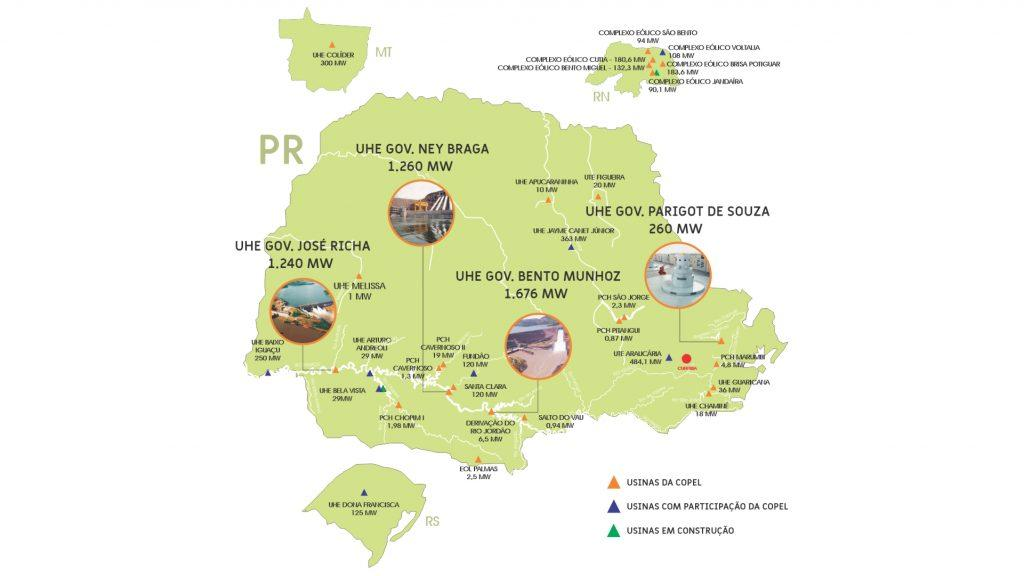
\includegraphics[width=1\linewidth]{img/usinas_copel} \caption{Usinas da Copel localizadas em mapa do Paraná.}\label{fig:unnamed-chunk-2}
  \end{figure}
  Comecemos comentando a respeito das hidrelétricas. Existe uma diferenciação entre Central Geradora Hidrelétrica (CGH), Pequena Central Hidrelétrica (PCH) e Usina Hidrelétrica (UHE). Por mais que todas se aproveitem do potencial hidráulico de um recurso hídrico, a diferença está no porte do empreendimento. Como disposto pela ANEEL, na Resolução n° 875, de 10 de março de 2020,\footnote{Disponível em: \url{https://www.in.gov.br/web/dou/-/resolucao-normativa-n-875-de-10-de-marco-de-2020-248070610}. Último acesso em 17 nov 2020.} a diferenciação é tal:
  \begin{itemize}
  \tightlist
  \item
    Uma \textbf{Central Geradora Hidrelétrica com Capacidade Instalada Reduzida (CGH)} é aquela cuja potência seja igual ou inferior a 5 MW.
  \item
    Uma \textbf{Pequena Central Hidrelétrica (PCH)} é aquela que possuem duas características: (1) potência instalada superior a 5 MW e igual ou inferior a 30 MW; e (2) área de reservatório de até 13 km², excluindo a calha do leito regular do rio. Existem, ainda, cláusulas que regularizam a condição de (2).
  \item
    Uma \textbf{Usina Hidrelétrica (UHE)} é aquela que possui quaisquer uma das seguintes características: (1) potência instalada superior a 5 MW e igual ou inferior a 50 MW, desde que não sejam enquadrados como PCH e estejam sujeitos à outorga de autorização; (2) potência instalada superior a 50 MW, sujeitos à outorga de concessão; ou (3) independente da potência instalada, tenham sido objeto de outorga de concessão ou de autorização.
  \end{itemize}
  Essa diferenciação é relevante, uma vez que o licenciamento destes três tipos de empreendimento ocorre de forma diferenciada. Isso decorre do fato que a extensão dos impactos ambientais provocados pelas CGHs, PCHs e UHEs são, também, diferenciados.

  Assim sendo, são as hidrelétricas tanto operacionais quanto em construção, com participação da Copel:
  \begin{itemize}
  \tightlist
  \item
    \textbf{UHE Colíder.} Está sendo construída na região norte do Mato Grosso, nos municípios de Nova Canaã do Norte e Itaúba. O empreendimento terá potência instalada estimada de 300 MW, o suficiente para atender ao consumo de uma cidade com 850 mil habitantes. Cabe comentar que essa obra é integrante do PAC do Governo Federal.
  \item
    \textbf{UHE Governador Ney Aminthas de Barros Braga,} anterior UHE Segredo. Esta é a segunda usina da Copel em potência instalada, com capacidade de 1.260 MW. Está localizada no rio Iguaçu, no município de Mangueirinha. Foi inaugurada em 1992, tendo sido a primeira UHE a possuir um Relatório de Impacto Ambiental (Rima) no Brasil.
  \item
    \textbf{UHE Governador José Richa,} anterior UHE Salto Caxias. É uma das mais importantes da Copel, tendo 1.240 MW de potência instalada. Foi inaugurada em fevereiro de 1999 e está situada no rio Iguaçu, no município de Capitão Leônidas Marques.
  \item
    \textbf{UHE Governador Bento Munhoz da Rocha Netto,} anterior UHE Foz do Areia. Esta é a maior usina da Copel, com capacidade instalada de 1.676 MW. Está localizada no rio Iguaçu, no município de Pinhão. Como um todo, a operação foi iniciada em 1980; suas operações causaram a desativação da PCH Salto Grande do Iguaçu, que contava com 15.2 MW.
  \item
    \textbf{UHE Baixo Iguaçu.} Tem capacidade instalada de 350,2 MW -- suficiente para atender uam cidade com 1 milhão de habitantes. Iniciou suas operações no primeiro semestre de 2019. A Copel detém 30\% de participação nesta usina instalada no rio Iguaçu, entre os municípios de Capanema e Capitão Leônidas Marques.
  \item
    \textbf{UHE Governador Pedro Viriato Parigot de Souza,} anterior UHE Capivari-Cachoeira. Possui potência de 260 MW, estando situada no município de Antonina, com reservatório localizado no município de Campina Grande do Sul. Entrou em operação em 1970, embora tenha sido inaugurada oficialmente em 26 de janeiro de 1971. Ela é a maior central subterrânea do sul do país.
  \item
    \textbf{UHE Dona Francisca.} Com potência instalada de 125 MW, a Copel detém participação de 23,03\% no capital social da Dona Francisca Energética S/A (Dfesa). Foi inaugurada em maio de 2001.
  \item
    \textbf{UHE Santa Clara.} Tem potência instalada de 120 MW, com garantia física de 69,6 MW médios. Está localizada entre os municípios de Candói e Pinhão, no rio Jordão. Conta, ainda, com uma PCH de potência 3,6 MW e garantia de 2,79 MW médios.
  \item
    \textbf{UHE Fundão.} Possui potência instalada de 120 MW, com garantia física de 65,8 MW médios. Está localizada próximo ao município de Pinhão. Conta, ainda, com uma PCH de potência 2,5 MW e garantia de 2,11 MW médios.
  \item
    \textbf{UHE Guaricana.} Possui potência de 36 MW. Localize-se na margem esquerda do rio Arraial, no município de Guaratuba. A usina foi adquirida pela Copel quando houve a incorporação da Cia. Força e Luz do Paraná, embora tenha sido inaugurada em 1957.
  \item
    \textbf{UHE Derivação do Rio Jordão.} Foi inaugurada em dezembro de 1997, com potência de 6,5 MW. Está localizada no município de Reserva do Iguaçu.
  \item
    \textbf{PCH São Jorge.} Possui capacidade instalada de 2,3 MW e está localizada à margem esquerda do rio Pintagui, numa região denominada Alagados. A usina foi inaugurada em 1945, na época pertencendo à Companhia Prada de Eletricidade S.A.; apenas em dezembro de 1974 foi incorporada pela Copel.
  \item
    \textbf{PCH Apucaraninha.} Tem capacidade instalada de 10 MW. Foi inaugurada em 1949, pela Empresa Elétrica de Londrina S.A., e incorporada pela Copel em 1974. Está localizada no município de Tamarana, na margem direita do rio Apucaraninha.
  \item
    \textbf{PCH Arturo Andreoli,} também conhecida como PCH Foz do Chopim. A Copel detém 35,77\% de participação societária da Foz do Chopim Energética Ltda., empresa constituída para exploração da PCH. Tem potência total instalada de 29,1 MW, e a usina como um todo entrou em operação comercial em novembro de 2001.
  \item
    \textbf{PCH Chaminé.} Possui capacidade instalada de 18 MW, e está localizada na margem esquerda do rio São João, no município de São José dos Pinhais. Foi construída pela Cia. Força e Luz do Paraná, começando a operar em 1930. Foi incorporada pela Copel em 1975.
  \item
    \textbf{PCH Cavernoso.} Esta possui a potência de 1,3 MW. Está localizada na margem direita do rio Cavernoso no município de Virmond. Interessantemente, ela opera a fio d'água, significando que a geração é feita apenas através da vazão normal do rio. Foi construída no final da década de 50 pelo DNAEE e pela prefeitura de Laranjeiras do Sul; entretanto foi inaugurada em 1965, quando foi incorporada pela Copel e teve sua capacidade ampliada.
  \item
    \textbf{PCH Cavernoso II.} Tem capacidade instalada de 19 MW, com garantia física de 10,6 MW médio. Foi construída no rio Cavernoso, entre os municípios de Virmond e Candói. A Central entrou em operação comercial a plena capacidade em 4 de julho de 2013.
  \item
    \textbf{PCH Chopim I.} Tem potência instalada de 1,98 MW e está localizada na margem esquerda do rio Chopim, no município de Itapejara d'Oeste. Foi a primeira usina construída pela Copel, durante a concepção do primeiro plano de eletrificação do Paraná. A operação começou em 1963.
  \item
    \textbf{PCH Bela Vista.} Está sendo instalada no rio Chopim, entre os municípios de Verê e São João, no sudoeste paranaense. O empreendimento recebeu do Instituto Ambiental do Paraná a Licença de Instalação nº 23.569, no dia 10 de maio de 2019. Quando estiver pronta, Bela Vista terá potência instalada de 29 MW e produzirá energia elétrica suficiente para atender até 100 mil pessoas.
  \item
    \textbf{CGH Salto do Vau.} Possui potência instalada de 0.94 MW e está localizada na margem esquerda do rio Palmital, no município de União da Vitória. Foi inaugurada em 1959, quando começou a operar. Foi construída pela empresa Alexandre Schlemm e incorporada pela Copel em novembro de 1973.
  \item
    \textbf{CGH Pitangui.} Possui 0,87 MW de potência e está localizada na margem esquerda do rio Pitangui, a 12 km de Ponta Grossa. Foi construída por outra empresa em 1911, mas finalmente incorporada pela Copel em 1974.
  \item
    \textbf{CGH Melissa.} Possui capacidade de 1 MW de potência instalada e situa-se no município de Corbélia, à margem direita do rio Melissa. Efetivamente, sua operação iniciou-se em 1969, embora tenha sido pausada para uma reforma geral durante a implantação dos equipamentos que a tornaram automatizada em 1994. Retomou, então, a operação no segundo semestre de 1995.
  \item
    \textbf{CGH Marumbi.} Possui uma capacidade de 4,8 MW de potência em duas unidades geradores, e está localizada no município de Morretes, à margem direita do rio Ipiranga. Foi inaugurada em abril de 1961, construída pela RFFSA. Em razão do Plano Nacional de Desestatização, por não se enquadradar nas atividades da RFFSA, a usina foi adquirida pela Copel em novembro de 1997.
  \end{itemize}
  No que tange a usinas termelétricas, a Copel possui:
  \begin{itemize}
  \tightlist
  \item
    \textbf{UTE Figueira.} Conta com capacidade instalada dae 20 MW, e funciona a base carvão mineral extraído em jazidas da região. A aquisicação da usina foi feita pela Copel em 1969, com posterior instalação de um terceiro grupo gerador, em 1974.
  \item
    \textbf{UTE Araucária.} Com capacidade instalada de 484,5 MW, se faz valer de um ciclo combinado de turbina a gás/turbina a vapor para dispor energia. A usina entrou em operação em 2006 para atender ao SIN, em face da severa estiagem ocorrida no início do seguneto semestre do ano.
  \end{itemize}
  Vale comentar, entretanto, que a capacidade instalada das UTEs não deve ser tratada como algo sob ``uso constante'', como é o caso de UHEs, por exemplo. De fato, as UTEs servem atualmente mais como um mecanismo de segurança do sistema energético do que um método de produção regular, pelo alto custo da energia, assim como os problemas relativos à poluição e gases do efeito estufa (ROSA, \protect\hyperlink{ref-rosa2007}{2007}).

  Finalmente, no que tange a energia eólica, a Copel conta com:
  \begin{itemize}
  \tightlist
  \item
    \textbf{EOL Palmas.} É composta por cinco aerogerados de 500 kW cada, totalizando assim 2,5 MW de potência instalada. Está situada no município de Palmas, ao sul do Paraná. Foi a primeira eólica da região sul do Brasil. Entrou em operação em fevereiro de 1999, mas apenas em 2008 a Copel deteve adquiriu total controle da empresa responsável pela usina, a Centrais Eólicas do Paraná.
  \item
    \textbf{Complexo Eólico São Bento Energia.} Está localizado nos municípios de Pedra Grande e São Bento do Norte -- no Rio Grande do Norte. Tem 94 MW de potência instalada.
  \item
    \textbf{Complexo Eólico Brisa Potiguar.} Está localizado nos municípios de Parazinho, João Câmara e Touros -- no Rio Grande do Norte. Tem 183,6 MW de potência instalada.
  \item
    \textbf{Complexo Eólico Cutia.} Está localizado nos municípios de Pedra Grande e São Bento do Norte -- no Rio Grande do Norte. Tem 180,6 MW de potência instalada.
  \item
    \textbf{Complexo Eólico Bento Miguel.} Está localizado no município de São Bento do Norte -- no Rio Grande do Norte. Tem 132,3 MW de potência instalada.
  \item
    \textbf{Complexo Eólico Voltalia.} Está localizado nos municípios de São Miguel do Gostoso e Touros -- no Rio Grande do Norte. Conta com 108 MW de potência instalada.
  \end{itemize}
  Assim sendo, é possível observar que a matriz energética da Copel é diversificada com maior ênfase em hidrelétricas, com recentes desenvolvimentos na construção de parques eólicos, de forma a se aproveitar de Créditos de Carbono e uma fronte de energias mais limpas.

  \hypertarget{transmissuxe3o}{%
  \subsubsection{Transmissão}\label{transmissuxe3o}}

  Como uma \emph{holding}, a Copel também está presente no setor de transmissão de energia elétrica. De fato, referente a junho de 2016, a Copel possuía 2.521,2 km de linhas e 35 subestações, somando 13.002 MVA de potência de transformação.

  As tabelas abaixo apresentam o dimensionamento dos ativos de transmissão da Copel relativos à Rede Básica, para o período de junho de 2016. Cabe comentar que todas as subestações são inteiramente automatizadas.
  \begin{table}

  \caption{\label{tab:unnamed-chunk-3}Extensão de linhas de transmissão da Copel, por nível de tensão.}
  \centering
  \begin{tabular}[t]{cc}
  \toprule
  \multicolumn{2}{c}{\textbf{LINHAS DE TRANSMISSÃO}} \\
  \cmidrule(l{3pt}r{3pt}){1-2}
  NÍVEL DE TENSÃO (kV) & EXTENSÃO (km)\\
  \midrule
  69 & 0.0\\
  138 & 7.2\\
  230 & 2235.5\\
  525 & 278.5\\
  \bottomrule
  \end{tabular}
  \end{table}
  \begin{table}

  \caption{\label{tab:unnamed-chunk-4}Subestações de transmissão da Copel, por nível de tensão.}
  \centering
  \begin{tabular}[t]{ccc}
  \toprule
  \multicolumn{3}{c}{\textbf{SUBESTAÇÕES DE TRANSMISSÃO}} \\
  \cmidrule(l{3pt}r{3pt}){1-3}
  NÍVEL DE TENSÃO (kV) & QUANTIDADE & POTÊNCIA (MVA)\\
  \midrule
  230 & 31 & 9602\\
  525 & 4 & 3400\\
  \bottomrule
  \end{tabular}
  \end{table}
  adasdas
  \begin{figure}[H]
  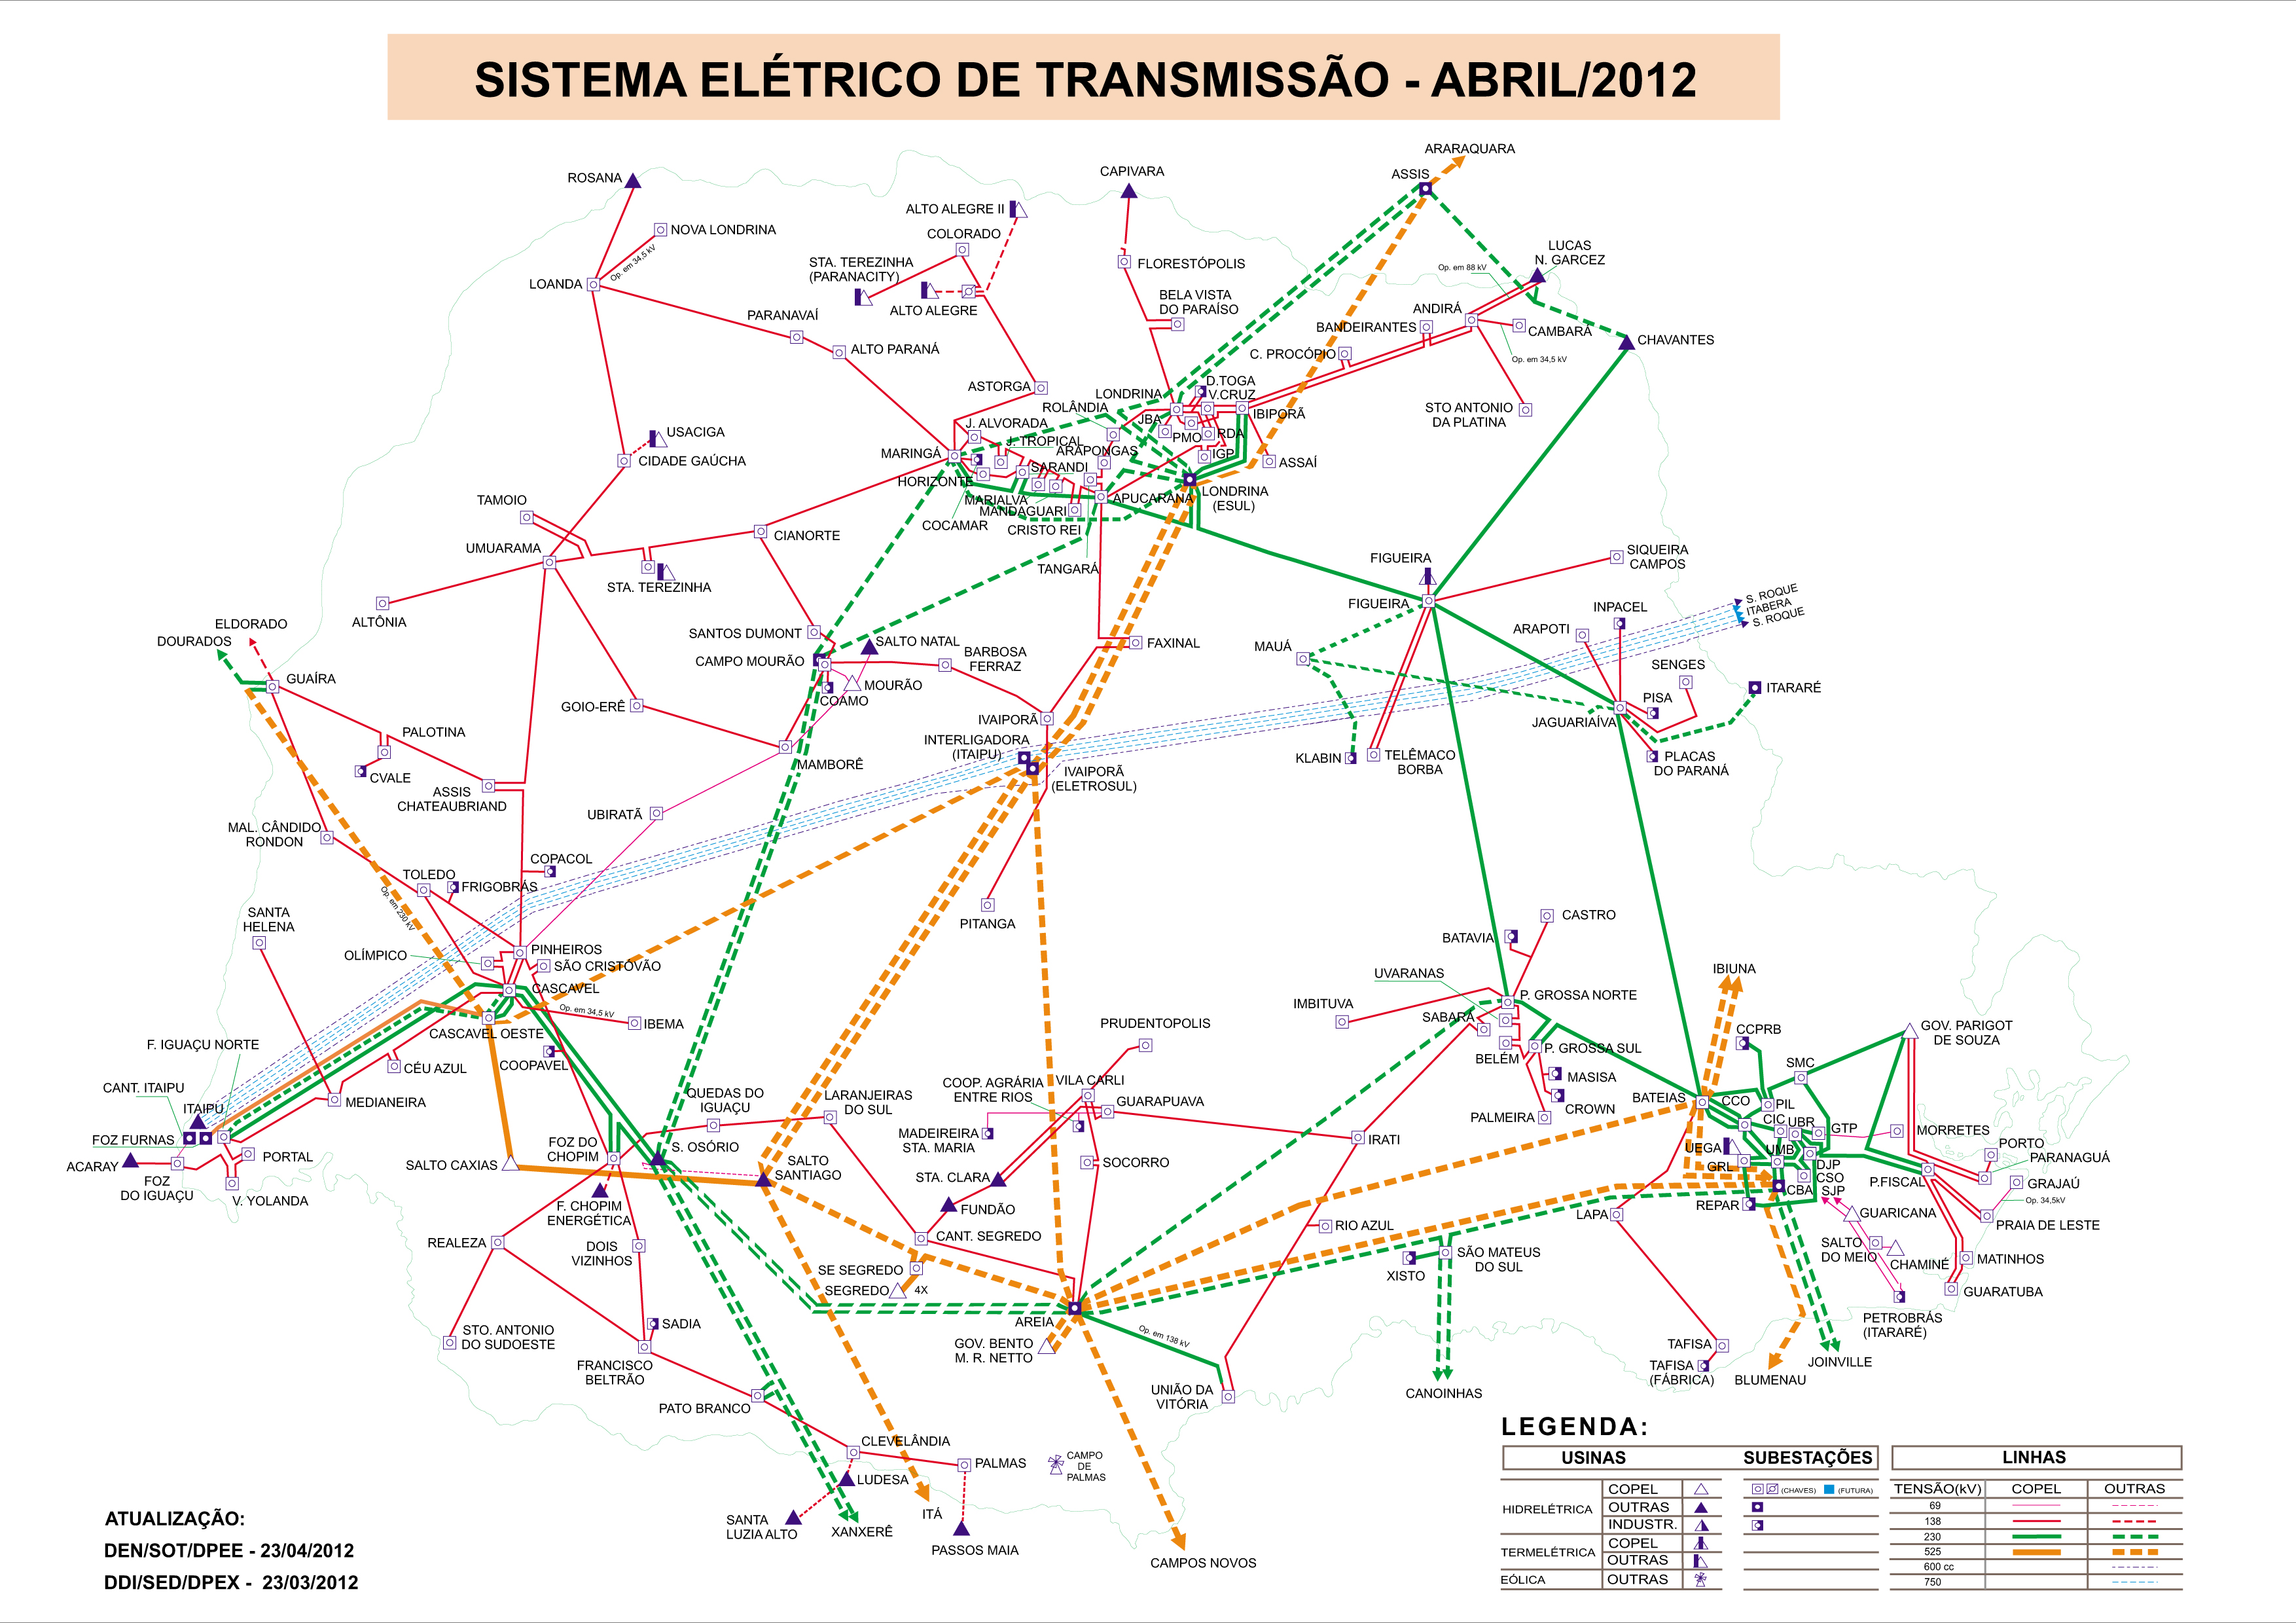
\includegraphics[width=1\linewidth]{img/mapa_geoeletrico_parana} \caption{Mapa geoelétrico do Paraná.}\label{fig:unnamed-chunk-5}
  \end{figure}
  \begin{figure}[H]
  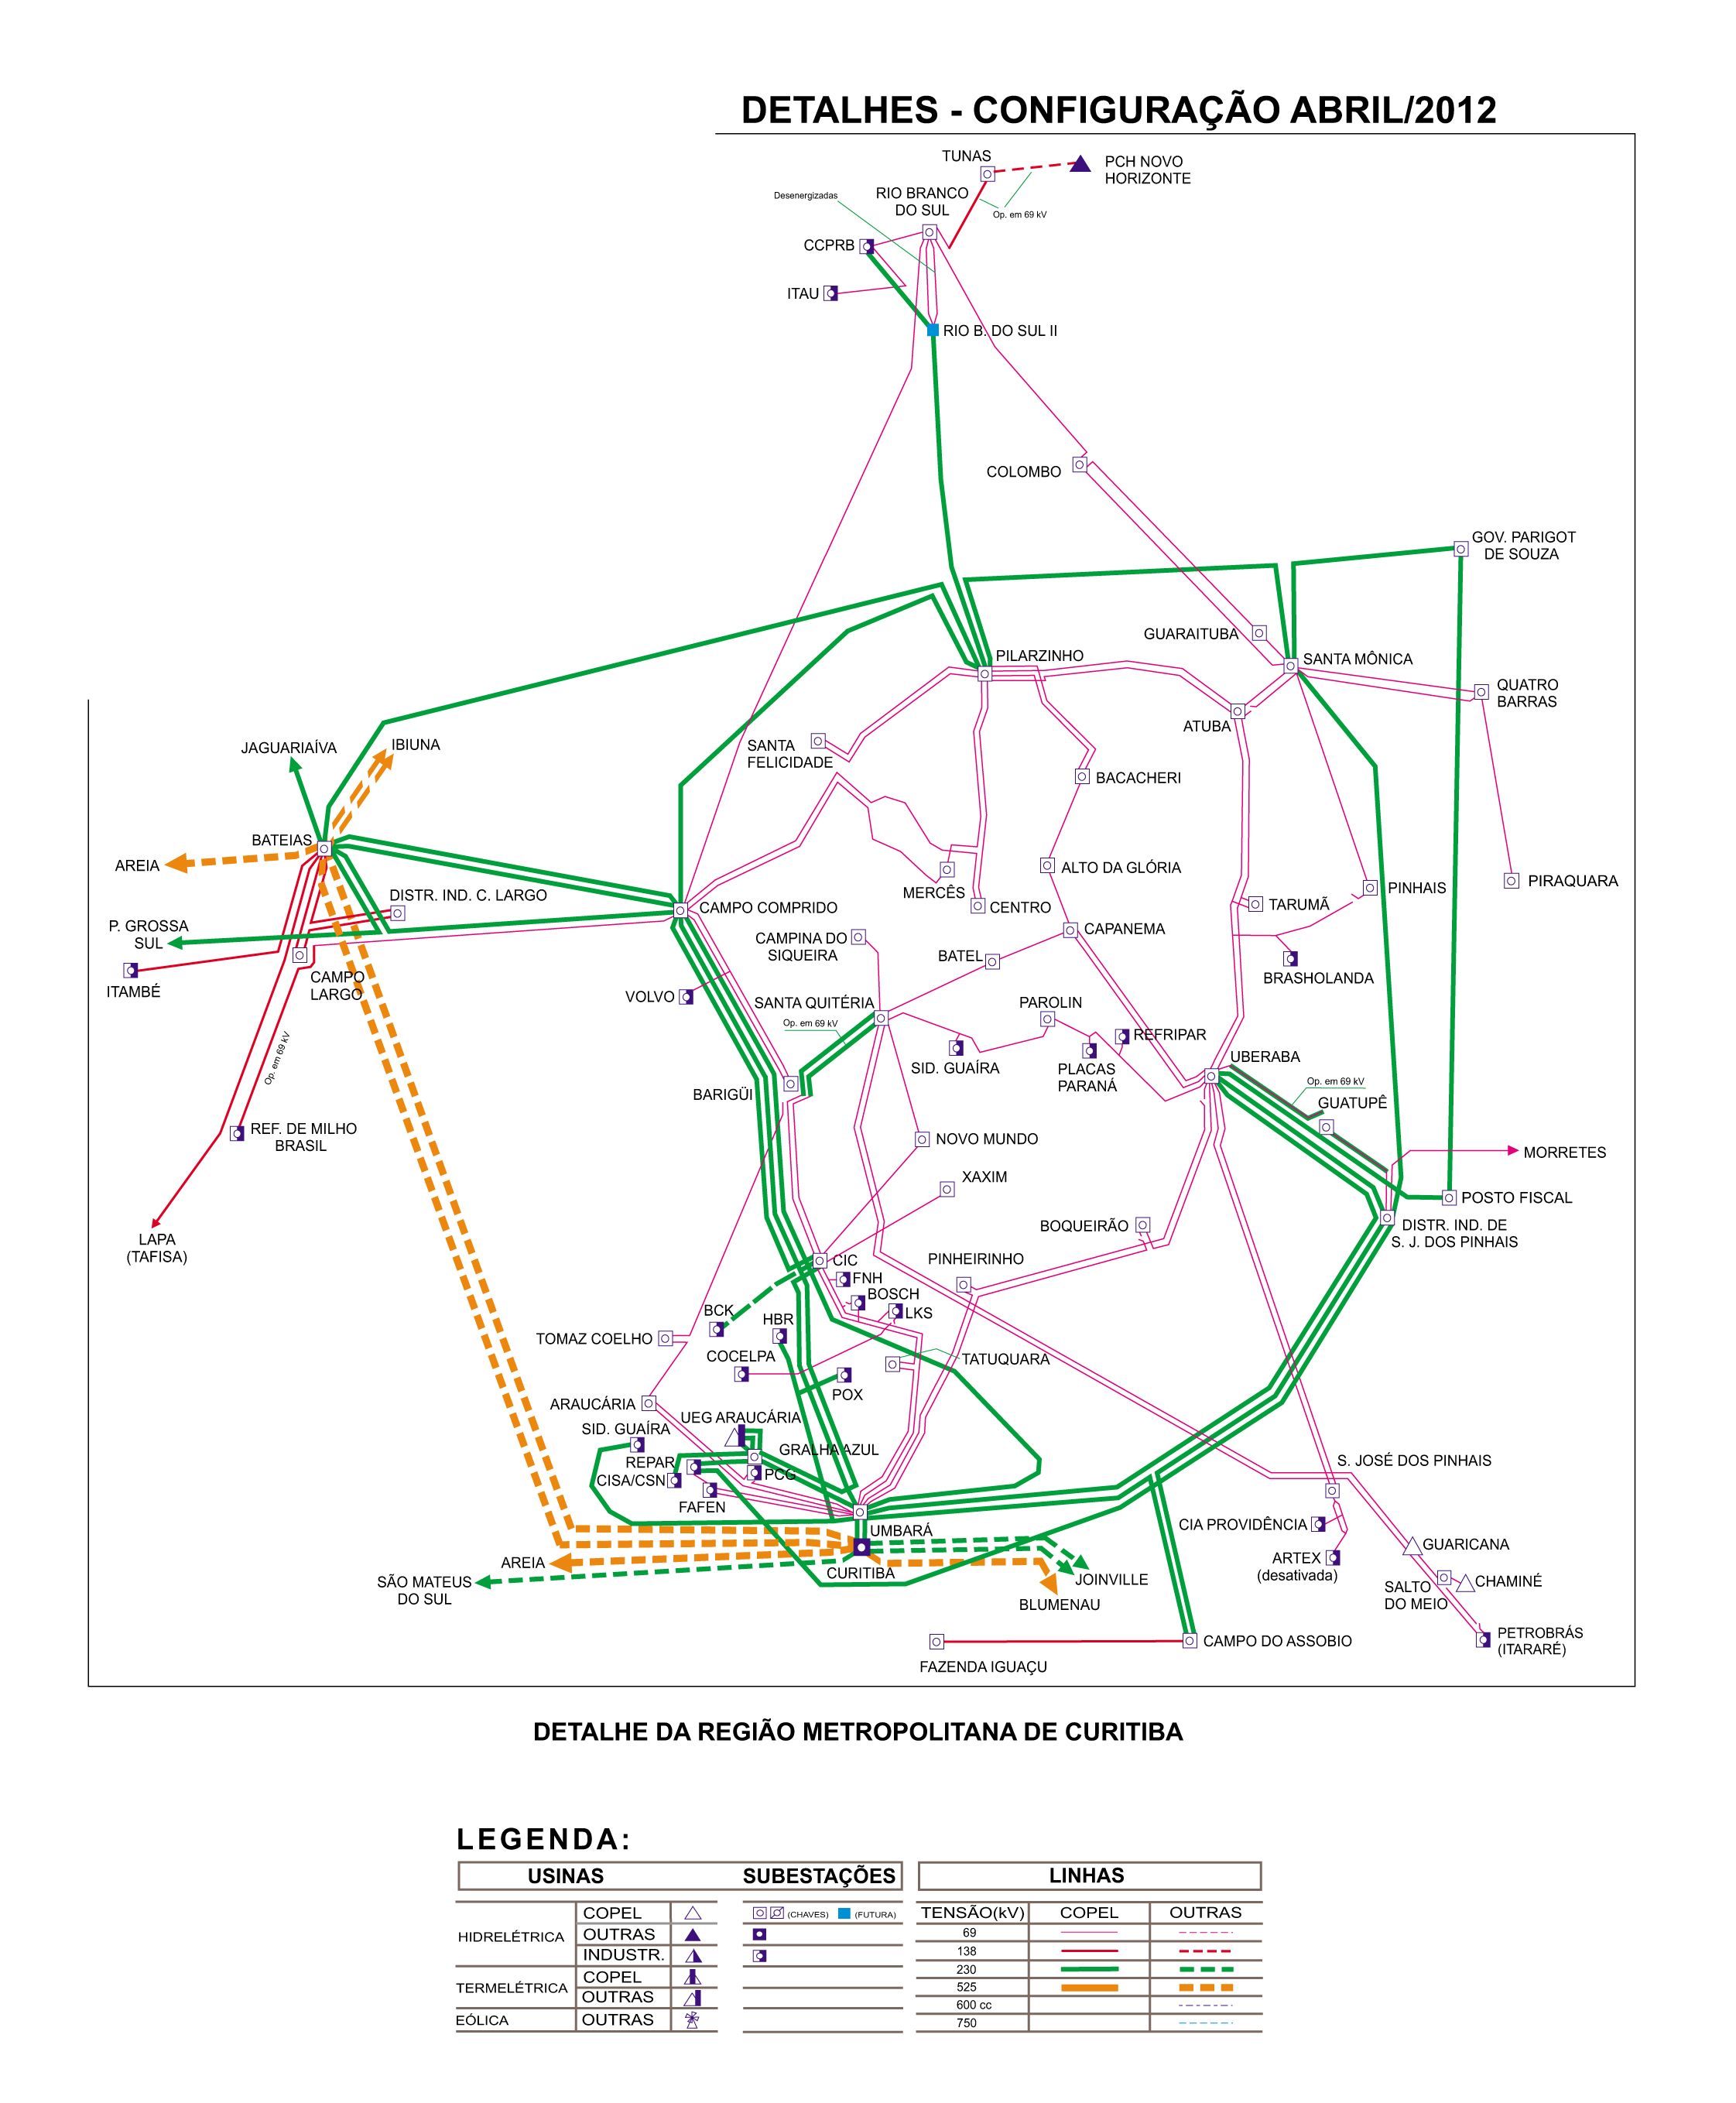
\includegraphics[width=1\linewidth]{img/mapa_geoeletrico_curitiba} \caption{Mapa geoelétrico de Curitiba.}\label{fig:unnamed-chunk-6}
  \end{figure}
  \begin{figure}[H]
  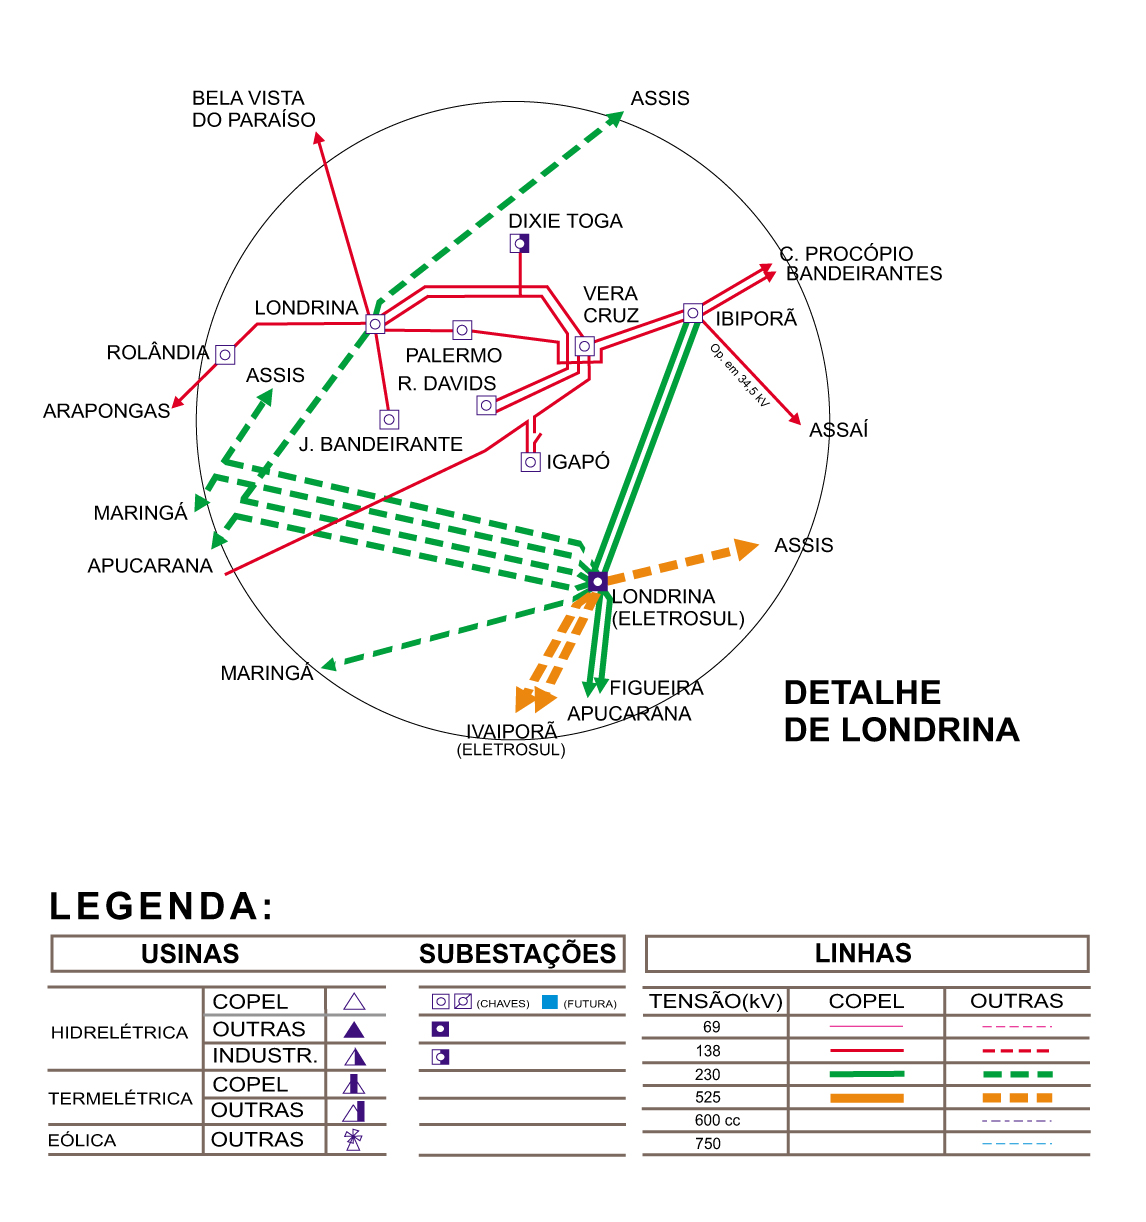
\includegraphics[width=1\linewidth]{img/mapa_geoeletrico_londrina} \caption{Mapa geoelétrico de Londrina.}\label{fig:unnamed-chunk-7}
  \end{figure}
  \begin{figure}[H]
  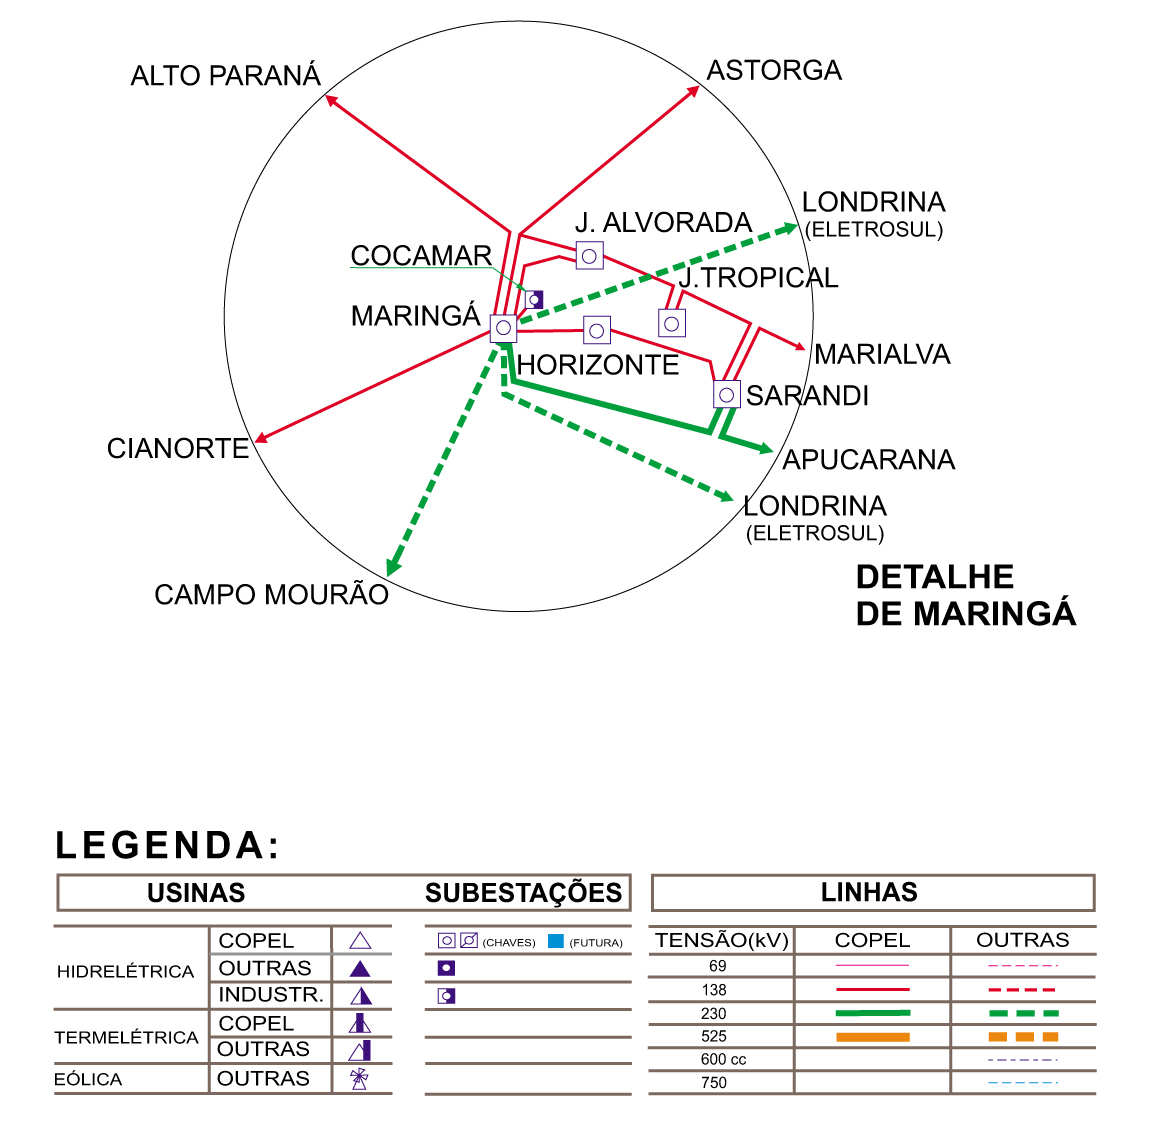
\includegraphics[width=1\linewidth]{img/mapa_geoeletrico_maringa} \caption{Mapa geoelétrico de Maringá.}\label{fig:unnamed-chunk-8}
  \end{figure}
  \begin{figure}[H]
  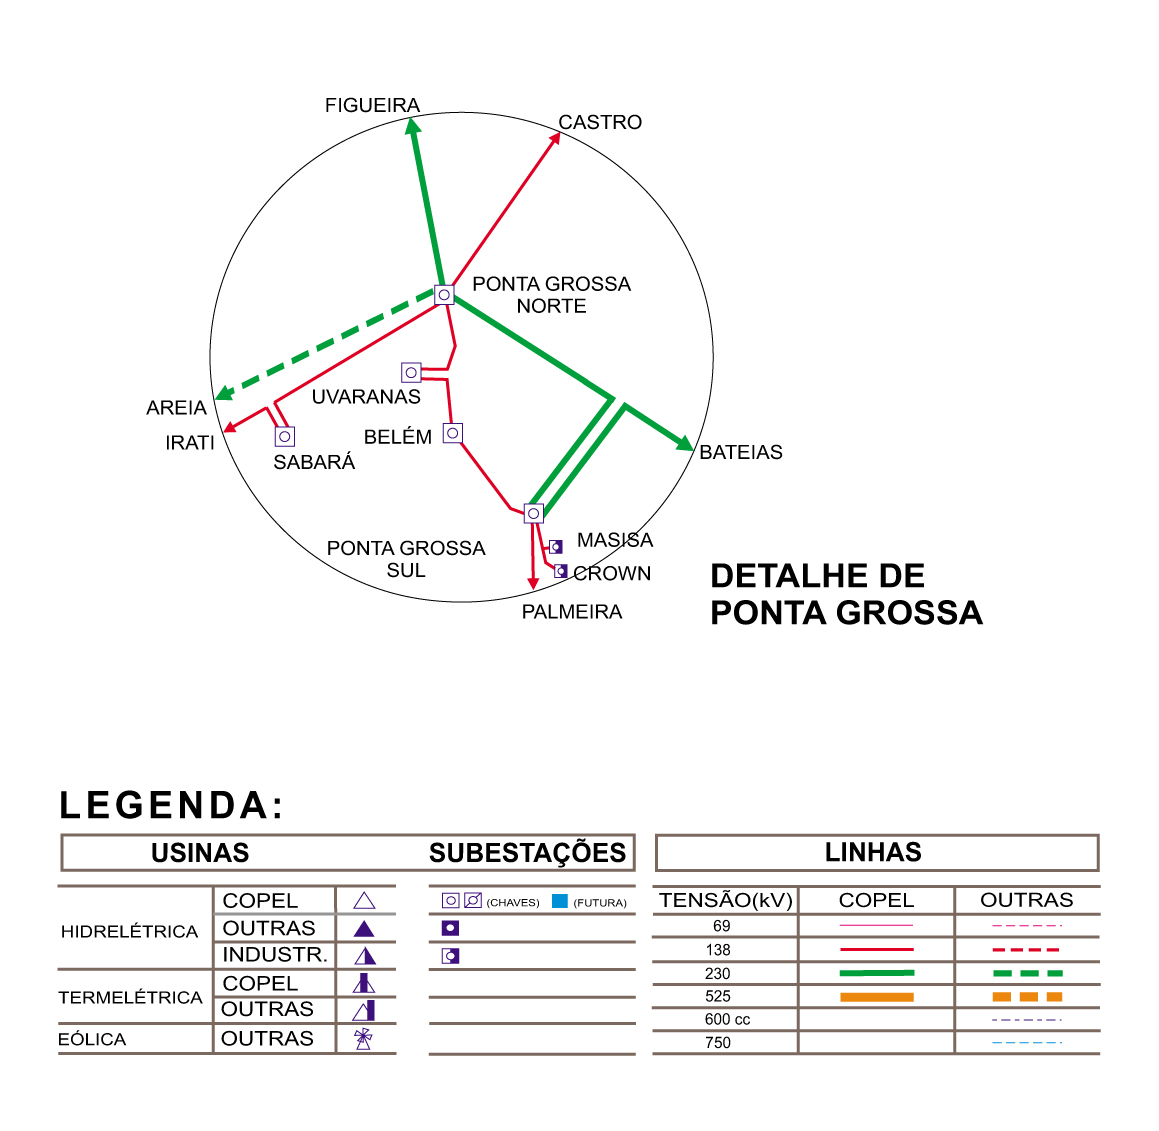
\includegraphics[width=1\linewidth]{img/mapa_geoeletrico_ponta_grossa} \caption{Mapa geoelétrico de Ponta Grossa.}\label{fig:unnamed-chunk-9}
  \end{figure}
  \hypertarget{distribuiuxe7uxe3o}{%
  \subsubsection{Distribuição}\label{distribuiuxe7uxe3o}}

  \hypertarget{cuxe1lculo-do-valuation-intruxednseco}{%
  \section{\texorpdfstring{Cálculo do \emph{valuation} intrínseco}{Cálculo do valuation intrínseco}}\label{cuxe1lculo-do-valuation-intruxednseco}}

  \hypertarget{o-custo-de-capital-muxe9dio-ponderado-wacc}{%
  \subsection{O custo de capital médio ponderado (WACC)}\label{o-custo-de-capital-muxe9dio-ponderado-wacc}}

  \hypertarget{custo-de-capital-pruxf3prio}{%
  \subsubsection{Custo de capital próprio}\label{custo-de-capital-pruxf3prio}}

  \hypertarget{custo-de-capital-de-terceiros}{%
  \subsubsection{Custo de capital de terceiros}\label{custo-de-capital-de-terceiros}}

  \hypertarget{fluxo-de-caixa-descontado}{%
  \subsubsection{Fluxo de caixa descontado}\label{fluxo-de-caixa-descontado}}

  \hypertarget{cuxe1lculo-do-valuation-relativo}{%
  \section{\texorpdfstring{Cálculo do \emph{valuation} relativo}{Cálculo do valuation relativo}}\label{cuxe1lculo-do-valuation-relativo}}

  \hypertarget{margem-bruta}{%
  \subsection{Margem bruta}\label{margem-bruta}}

  \hypertarget{lucros-antes-de-juros-e-impostos-ebit}{%
  \subsection{Lucros antes de juros e impostos (EBIT)}\label{lucros-antes-de-juros-e-impostos-ebit}}

  \hypertarget{margem-luxedquida}{%
  \subsection{Margem líquida}\label{margem-luxedquida}}

  \hypertarget{razuxe3o-preuxe7olucro-pe}{%
  \subsection{Razão preço/lucro (P/E)}\label{razuxe3o-preuxe7olucro-pe}}

  \hypertarget{retorno-sobre-patrimuxf4nio-luxedquido-roe}{%
  \subsection{Retorno sobre patrimônio líquido (ROE)}\label{retorno-sobre-patrimuxf4nio-luxedquido-roe}}

  \hypertarget{comparauxe7uxe3o-com-empresas-do-setor}{%
  \subsection{Comparação com empresas do setor}\label{comparauxe7uxe3o-com-empresas-do-setor}}

  \hypertarget{conclusuxe3o}{%
  \chapter{Conclusão}\label{conclusuxe3o}}

  \backmatter

  \hypertarget{referuxeancias-bibliogruxe1ficas}{%
  \chapter*{Referências Bibliográficas}\label{referuxeancias-bibliogruxe1ficas}}
  \addcontentsline{toc}{chapter}{Referências Bibliográficas}

  \markboth{References}{References}

  \label{bib:begin}
  \noindent

  \setlength{\parindent}{-0.20in}
  \setlength{\leftskip}{0.20in}
  \setlength{\parskip}{8pt}

  \hypertarget{refs}{}
  \begin{cslreferences}
  \leavevmode\hypertarget{ref-anbima2019}{}%
  ANBIMA. \textbf{Raio-X do Investidor Brasileiro}, 2019.

  \leavevmode\hypertarget{ref-arnold2008}{}%
  ARNOLD, G. \textbf{Corporate financial management}. New York City, NY: Pearson Education, 2008.

  \leavevmode\hypertarget{ref-beaver1970}{}%
  BEAVER, W.; KETTLER, P.; SCHOLES, M. The association between market determined and accounting determined risk measures. \textbf{The Accounting Review}, v. 45, n. 4, p. 654--682, 1970.

  \leavevmode\hypertarget{ref-beaver1978}{}%
  BEAVER, W.; MORSE, D. What determines price-earnings ratios? \textbf{Financial Analysts Journal}, v. 34, n. 4, p. 65--76, 1978.

  \leavevmode\hypertarget{ref-bogle2015}{}%
  BOGLE, J. C. \textbf{Bogle on mutual funds: New perspectives for the intelligent investor}. New Jersey: John Wiley \& Sons, 2015.

  \leavevmode\hypertarget{ref-damodaran2007}{}%
  DAMODARAN, A. \textbf{Valuation approaches and metrics: a survey of the theory and evidence}. {[}s.l.{]} Now Publishers Inc, 2007.

  \leavevmode\hypertarget{ref-damodaran2012}{}%
  DAMODARAN, A. \textbf{Investment philosophies: successful strategies and the investors who made them work}. Hoboken, NJ: John Wiley \& Sons, 2012.

  \leavevmode\hypertarget{ref-epe2020}{}%
  EPE. \textbf{Plano Nacional de Energia 2050}. Brasília: Ministério de Minas e Energia, 2020.

  \leavevmode\hypertarget{ref-fama2004}{}%
  FAMA, E. F.; FRENCH, K. R. The capital asset pricing model: Theory and evidence. \textbf{Journal of economic perspectives}, v. 18, n. 3, p. 25--46, 2004.

  \leavevmode\hypertarget{ref-fisher1930}{}%
  FISHER, I. \textbf{Theory of interest: as determined by impatience to spend income and opportunity to invest it}. New York City, NY: Augustusm Kelly Publishers, Clifton, 1930.

  \leavevmode\hypertarget{ref-techreport-exampleIn}{}%
  GARRET, D. A. \textbf{The Microscopic Detection of Corrosion in Aluminum Aircraft Structures with Thermal Neutron Beams and Film Imaging Methods}. Washington, D.C.: National Bureau of Standards, 1977.

  \leavevmode\hypertarget{ref-gordon1959}{}%
  GORDON, M. J. Dividends, earnings, and stock prices. \textbf{The review of economics and statistics}, p. 99--105, 1959.

  \leavevmode\hypertarget{ref-gordon1956}{}%
  GORDON, M. J.; SHAPIRO, E. Capital equipment analysis: the required rate of profit. \textbf{Management science}, v. 3, n. 1, p. 102--110, 1956.

  \leavevmode\hypertarget{ref-graham2016}{}%
  GRAHAM, B. \textbf{O investidor inteligente}. Rio de Janeiro: HarperCollins Brasil, 2016.

  \leavevmode\hypertarget{ref-article-example}{}%
  IESAN, D. Existence Theorems in the Theory of Mixtures. \textbf{Journal of Elasticity}, v. 42, n. 2, p. 145--163, fev. 1996.

  \leavevmode\hypertarget{ref-klayman1995}{}%
  KLAYMAN, J. Varieties of confirmation bias. \textbf{Psychology of learning and motivation}, v. 32, p. 385--418, 1995.

  \leavevmode\hypertarget{ref-kruger1999}{}%
  KRUGER, J.; DUNNING, D. Unskilled and unaware of it: how difficulties in recognizing one's own incompetence lead to inflated self-assessments. \textbf{Journal of personality and social psychology}, v. 77, n. 6, p. 1121, 1999.

  \leavevmode\hypertarget{ref-lie2002}{}%
  LIE, E.; LIE, H. J. Multiples used to estimate corporate value. \textbf{Financial Analysts Journal}, v. 58, n. 2, p. 44--54, 2002.

  \leavevmode\hypertarget{ref-liu2002}{}%
  LIU, J.; NISSIM, D.; THOMAS, J. Equity valuation using multiples. \textbf{Journal of Accounting Research}, v. 40, n. 1, p. 135--172, 2002.

  \leavevmode\hypertarget{ref-liu2007}{}%
  LIU, J.; NISSIM, D.; THOMAS, J. Is cash flow king in valuations? \textbf{Financial Analysts Journal}, v. 63, n. 2, p. 56--68, 2007.

  \leavevmode\hypertarget{ref-markowitz1952}{}%
  MARKOWITZ, H. Portfolio selection. \textbf{The Journal of Finance}, v. 7, n. 1, p. 77--91, 1952.

  \leavevmode\hypertarget{ref-modigliani1958}{}%
  MODIGLIANI, F.; MILLER, M. H. The cost of capital, corporation finance and the theory of investment. \textbf{The American economic review}, v. 48, n. 3, p. 261--297, 1958.

  \leavevmode\hypertarget{ref-munger2006}{}%
  MUNGER, C. T. \textbf{Poor Charlie's Almanack: The Wit and Wisdom of Charles T. Munger}. Virginia Beach: Donning Company, 2006.

  \leavevmode\hypertarget{ref-assafneto2018}{}%
  NETO, A. A. \textbf{Mercado financeiro}. 14. ed. São Paulo: Atlas, 2018.

  \leavevmode\hypertarget{ref-peasnell1982}{}%
  PEASNELL, K. V. Some formal connections between economic values and yields and accounting numbers. \textbf{Journal of Business Finance \& Accounting}, v. 9, n. 3, p. 361--381, 1982.

  \leavevmode\hypertarget{ref-penman1996}{}%
  PENMAN, S. H. The articulation of price-earnings ratios and market-to-book ratios and the evaluation of growth. \textbf{Journal of accounting research}, v. 34, n. 2, p. 235--259, 1996.

  \leavevmode\hypertarget{ref-rosa2007}{}%
  ROSA, L. P. Geração hidrelétrica, termelétrica e nuclear. \textbf{Estudos Avançados}, v. 21, n. 59, p. 39--58, 2007.

  \leavevmode\hypertarget{ref-schwarz1991}{}%
  SCHWARZ, N. et al. Ease of retrieval as information: another look at the availability heuristic. \textbf{Journal of Personality and Social psychology}, v. 61, n. 2, p. 195, 1991.

  \leavevmode\hypertarget{ref-sharpe1964}{}%
  SHARPE, W. F. Capital asset prices: A theory of market equilibrium under conditions of risk. \textbf{The journal of finance}, v. 19, n. 3, p. 425--442, 1964.

  \leavevmode\hypertarget{ref-simon1997}{}%
  SIMON, H. A. \textbf{Models of bounded rationality: Empirically grounded economic reason}. Massachusetts: MIT press, 1997. v. 3

  \leavevmode\hypertarget{ref-stohs1996}{}%
  STOHS, M. H.; MAUER, D. C. The determinants of corporate debt maturity structure. \textbf{Journal of business}, p. 279--312, 1996.

  \leavevmode\hypertarget{ref-wilcox1984}{}%
  WILCOX, J. W. The P/B-roe valuation model. \textbf{Financial Analysts Journal}, v. 40, n. 1, p. 58--66, 1984.
  \end{cslreferences}
  \backmatter
  \bibliographystyle{coppe-unsrt}
  \bibliography{thesis}

  %\appendix
  %\include{appenA}
\end{document}
